%set document class:
\documentclass[11pt,letterpaper]{article}

%configure page margins with geometry package:
\usepackage[left=1.in,right=1.in,footskip=0.5in,bottom=0.5in,top=0.5in,includefoot]{geometry}

%set language (load hyphenation patterns):
\usepackage[english]{babel}

%fonts and input encoding packages:
\usepackage[T1]{fontenc}
\usepackage{lmodern}
\usepackage[utf8]{inputenc}
\usepackage{indentfirst}

%graphics/figures packages:
\usepackage{graphicx}
\usepackage[usenames,dvipsnames]{color}
\usepackage{epstopdf}
\usepackage[labelfont=bf,hypcap=true]{caption}
\usepackage{subcaption}
\usepackage[title]{appendix}
\usepackage[section]{placeins}

%load additional (math) fonts:
\usepackage{amsmath}
\usepackage{amsfonts}
\usepackage{amssymb}
\usepackage{bm}
\usepackage{braket}
\usepackage{algorithm}
\usepackage[noend]{algpseudocode}
\makeatletter
\def\BState{\State\hskip-\ALG@thistlm}
\makeatother

%improve spacing between words and letters:
\usepackage{microtype}

%configure cross-references and links:
\usepackage{url}
%(set colorlinks=false to remove colored links)
\usepackage[hyperfootnotes=false,colorlinks=true,citecolor=Blue,
            urlcolor=Blue,linkcolor=Blue,breaklinks=true]{hyperref}

\usepackage{multicol}

%define some additional commands for convenience:
\title{KCore Paper}
%tensor/matrix:
\newcommand{\ten}[1]{\mathsf{#1}}
%vector with bold font:
\renewcommand{\vec}[1]{\mathbf{#1}}
%bold symbol (e.g. for greek letters):
\newcommand{\bs}[1]{\boldsymbol{#1}}
%differential:
\newcommand{\dd}{\,\mathrm{d}}
%partial differential:
\newcommand{\pd}{\partial}
%complex i:
\newcommand{\ii}{\mathrm{i}}


%all content goes between \begin{document} and \end{document}:
\begin{document}

%set title, author, and date:

%\title{\textsc{\large{K-Core Paper}}}  %\\ is for new line
\author{authors}
%\date{\today}
%make title:
\maketitle

%State the problem more clearly
\section{Introduction}
%The billions of neurons in the human brain form an incredibly complex circuit which is not completely understood. Instead, our focus can be turned to smaller networks within the brain, in hopes to better understand how specific subsystems govern the physical systems of the body. At its most basic level, a neuron is a component which receives an input signal, and outputs a signal. More specifically, input signals are received from other neurons from wide-branching tree-like structures called dendrites. Depending on the input signal received, different neurons produce different output signals which are then received as inputs by other neurons \cite{koch}.\\

The \textit{preB{\"o}tzinger Complex} was found to contain the oscillator responsible for the driving of inspiratory lung activity \cite{feldman_del_negro}. Prior to this relatively recent discovery, the precise network structure responsible for the generation of breathing rhythms was long unknown. A 1991 paper by Smith et al. proposed that the respiratory rhythm may originate from a structure of pacemaker cells in the \textit{preB{\"o}tzinger Complex}, a relatively small network of neurons located in mammallian brainstems \cite{preBotzinger_paper}. Subsequently, Feldman and del Negro suggested the mechanism by which this network produces the mammalian breathing rhythm \cite{feldman_del_negro}. Specifically, they proposed that two coupled oscillators in the brain control the cyclical breathing pattern in mammals. The \textit{preB{\"o}tzinger Complex} being responsible for inspiratory behavior, and the retrotrapezoid nucleus/parafacial respiratory group responsible for expiratory behavior \cite{feldman_del_negro}. A recent finding by Schwab et al. determined that the behavior of the network is in fact governed by an emergent leading cluster of interconnected neurons which drive its oscillatory behavior \cite{kcore_paper}.\\

To explain this emergent leading cluster, the concept of a k-core was introduced, which will be the centerpiece of our investigation of the network. The concept of a k-core was originally suggested in a discussion of social networks to describe the cohesiveness of an interconnected graph. Formally, it is defined as the maximally connected subgraph $H$ of a graph $G$ where each point of $H$ is adjacent to at least $\delta (H)$ other points of $H$, where $\delta (H)$ is the minimum degree of $H$ \cite{network_structure_minimum_degree}. Here, the term degree is defined as the number of connections a point receives. Interestingly, the k-core plays an important role in the network behavior of the \textit{preB{\"o}tzinger Complex}. In particular, the phase transition from a stably oscillating network to a phase diagram with a fixed point was found to correspond very well with k-core transitions \cite{kcore_paper}.\\

In this paper, we hope to establish a highly simplified model of the network dynamics of neurons in the \textit{preB{\"o}tzinger Complex} in order investigate the significance of emerging k-cores. Whereas previous investigations of the network's behavior relied on fermi and sigmoid functions with a sharp transition \cite{kcore_paper} slope to model the firing rate and calcium concentration of neurons in the network, we study the limit where these transitions are so sharp they become step functions. We first analyze the mean field limit of the network, and then proceed with a heterogeneously connected network. We find that, as a function of just a few parameters of the network, the exact size of the largest k valued k-core in the network can be determined to a high degree of accuracy. In analyzing the phase diagrams of these networks, we reproduce the results of the previous works by Schwab et al. Furthermore, we observe the same correspondence between k-core size and discontinuities in the phase diagram, which take on the form of discrete steps rather than a smooth function, despite using a simplified model. This suggests that the behavior of the network is very closely related to the most highly connected component within the network.\\

%A detailed investigation of the behavior of this network could prove to be of particular importance to studies of neurodegenerative disorders affecting breathing. Furthermore, by accurately modeling the emergent properties of the network, the precise mechanisms leading to the failure of the network to regulate breathing may be elucidated.\\

\section{A Simplified Model}
Neuron networks can be discussed mathematically through the language of graph theory. In particular, we show how we can go from an image of the \textit{preB{\"o}tzinger Complex} to a mathematical graph that encapsulates the significant features of the network (fig. \ref{fig:preBotzinger_anatomy}). While the adjacency matrix only contains information about the connectivity of the network, several other parameters can be defined do model the actual dynamics of the networks.

\begin{figure}[!htb]
	\centering
    	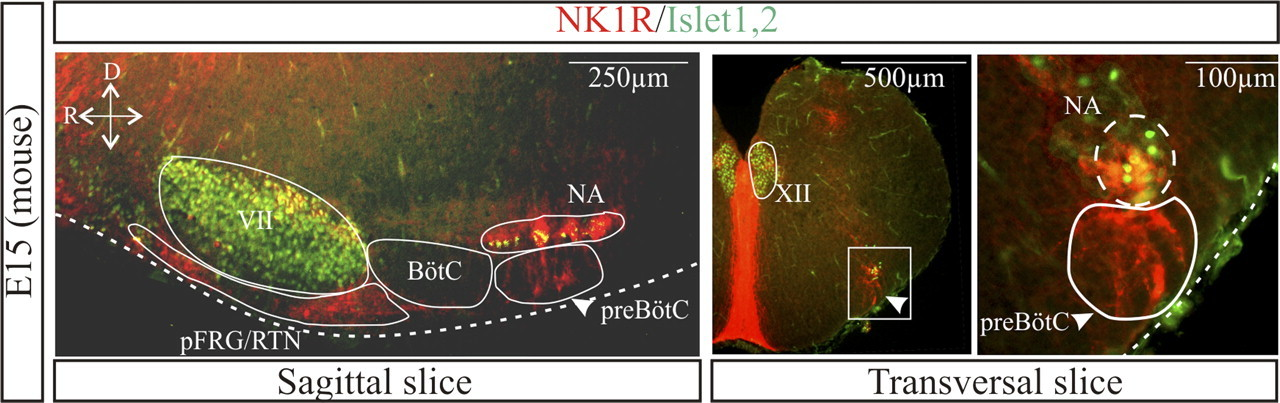
\includegraphics[width=100mm]{prebotzinger_image.jpeg}\\
        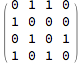
\includegraphics[width=30mm]{mat_test.png}
        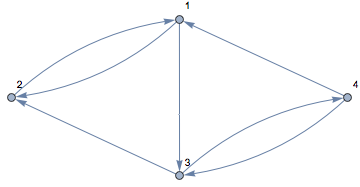
\includegraphics[width=70mm]{adj_mat_sample.png}
    \caption{Top: Image of mouse hindbrain slice containing network \cite{preBotzinger_anatomy}. Left: 4x4 adjacency matrix of 1's and 0's describing directed graph. Each row corresponds to a neuron, and the value in each column corresponds to a connection (1) or nonconnection (0) that it makes with another neuron. Right: Directed graph depiction of adjacency matrix.}
    \label{fig:preBotzinger_anatomy}
\end{figure}

We study neurons in the \textit{preB{\"o}tzinger Complex} with the integrate and fire model \cite{koch}, where each neuron takes an input signal, and as a function of the voltage received, produces an output signal. Consequently, a mathematical model for this kind of neuron demands the definition of firing rate as a function of input voltage, and a definition of voltage increment as a function of local calcium concentration. The rise in Ca$^{2+}$ has an inhibitory effect on other synaptic inputs into the cell, depolarizing it and effectively terminating the burst \cite{kcore_paper}. A "two-compartment" model for the neuronal network behavior of the \textit{preB{\"o}tzinger Complex} was proposed by Schwab et al\cite{kcore_paper}, whereby the dynamics of the network can be described by graph theory methods. %Revisit this last sentence
\begin{equation}
\label{eq:voltage_increment}
\frac{dV_i}{dt}=\frac{1}{\tau _V}(V_\text{eq}-V_i) + \Delta V(C_i)\sum _{j \neq i}M_{ij}P(V_j)
\end{equation}

\begin{equation}
\label{eq:calcium_increment}
\frac{dC_i}{dt}=\frac{1}{\tau _C}(C_\text{eq} - C_i) + \Delta C\sum _{j \neq i}M_{ij}P(V_j)
\end{equation}

In this model, each neuron was represented by two variables, $V_i(t)$ and $C_i(t)$, respectively indicating the somatic potential and average \textit{dendritic} Ca$^{2+}$ concentration of the $i$th neuron \cite{kcore_paper}. Here, $V_\text{eq}$ and $C_\text{eq}$ represent each neuron's resting potential and equilibrium Ca$^{2+}$ concentrations. $\tau_V$(10 ms) and $\tau_C$ (500 ms) \cite{koch} represent their respective equalizing time constants\cite{kcore_paper}. $M_{ij}$ represents the $i,j$'th entry of the adjacency matrix. To compute the voltage input into a neuron, the sum of voltages from all incoming neurons is considered. The bursting firing rate these neurons is modeled by equation \ref{eq:sigmoid_firing_rate}.

\begin{equation}
\label{eq:sigmoid_firing_rate}
P(V) = \frac{r_m-r_b}{1+e^{-(V-V*)/g_V}}+r_b
\end{equation}

Here, $r_m = 75$ Hz is the maximum neuron firing rate, $r_b = 5$ Hz is the minimal firing rate, and $V^* = -55$ mV is the activation voltage at which the neuron transitions to active firing \cite{kcore_paper}. The steepness of the activation function is determined by the constant $g_V = 5$ mV.

The second equation represents the calcium dependent voltage increment, which suppresses the voltage input and transitions the neuron from from its active firing rate to its minimal firing rate \cite{kcore_paper}. This was also modeled by a sigmoid function:

\begin{equation}
\label{eq:sigmoid_calcium_rate}
\Delta V(C)=\frac{\Delta V_{max}}{1+e^{(C-C*)/g_C}}
\end{equation}

%This doesn't belong here but it's important to discuss somewhere nevertheless.
One major discovery of this work was that the discontinuities of the phase boundary along the SO-Q and SO-HA phases using an Erdos-Renyi random network corresponded well with with k-core transitions \cite{kcore_paper}. Though this representation was in itself a simplification of the Feldman and Del Negro model, a further simplification can be made to the model by using a Heaviside step function activation function in place of Fermi functions. In effect, we take equations \ref{eq:sigmoid_firing_rate} and \ref{eq:sigmoid_calcium_rate} in the limit of very small $g_V$ and $g_C$, which sharpens the transition slope to a step. The step function offers the benefit of having the simplest model of a neuron activation function, either a pre-defined low voltage, or high voltage.\\

While the "two-compartment" model seemed to suggest that the network transitions from stable oscillations to fixed points by removing neurons from the network, the step function model suggests a different type of behavior of the network. In particular, in our computer simulations, the first neurons to transition from a bursting firing rate to the basal firing rate are the most highly connected ones, suggesting that it is in fact the most highly connected neurons in the network that stop firing. This is perhaps due to an oversaturation of Ca$^{2+}$ which has an inhibitory effect on other synaptic inputs.

\section{Mean Field Analysis of Simplified Model (Step Function)}
We seek to determine if any information about the connectivity of neurons in the \textit{preB{\"o}tzinger Complex} can be retrieved by using even more simplified voltage and calcium increment functions. We study the following functions in the mean field limit:

\begin{equation}
\label{eq:step_voltage_increment}
\dot{V} = -\frac{V}{\tau _v} + n [(\Delta V_1 - \Delta V_0) \theta (C^* - C) + \Delta V_0 ][r_1\theta (V - V^*) + r_0]
\end{equation}

\begin{equation}
\label{eq:step_calcium_increment}
\dot{C} = -\frac{C}{\tau _c} + n\Delta C [(r_1 - r_0) \theta (V - V^*) + r_0]
\end{equation}

Here, equations \ref{eq:sigmoid_firing_rate} and \ref{eq:sigmoid_calcium_rate} are incorporated into the voltage and calcium increment functions directly. The new variables introduced are $r_0$ and $r_1$. $r_0$ represents the basal firing rate, whereas $r_1 + r_0$ represents the active firing rate. Additionally, $n$ represents the number of neurons in the network in the mean field case, where every neuron receives voltage inputs from every other neuron. The assumptions of this fully connected network are that connections are not bi-directional, and the neurons are not directly connected to themselves. In order to observe stable oscillations, we require that the step function representing the firing rate has some offset from 0 (fig. \ref{fig:step_figures}).

\begin{figure}
	\centering
    	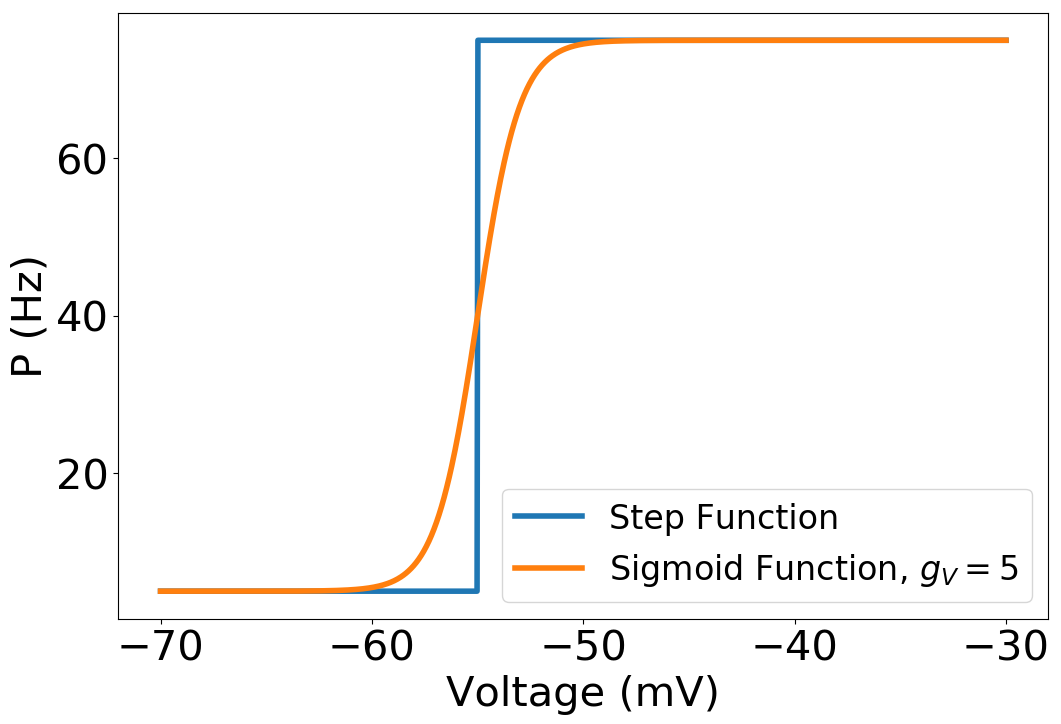
\includegraphics[width=65mm]{firing_rate_step.png}
        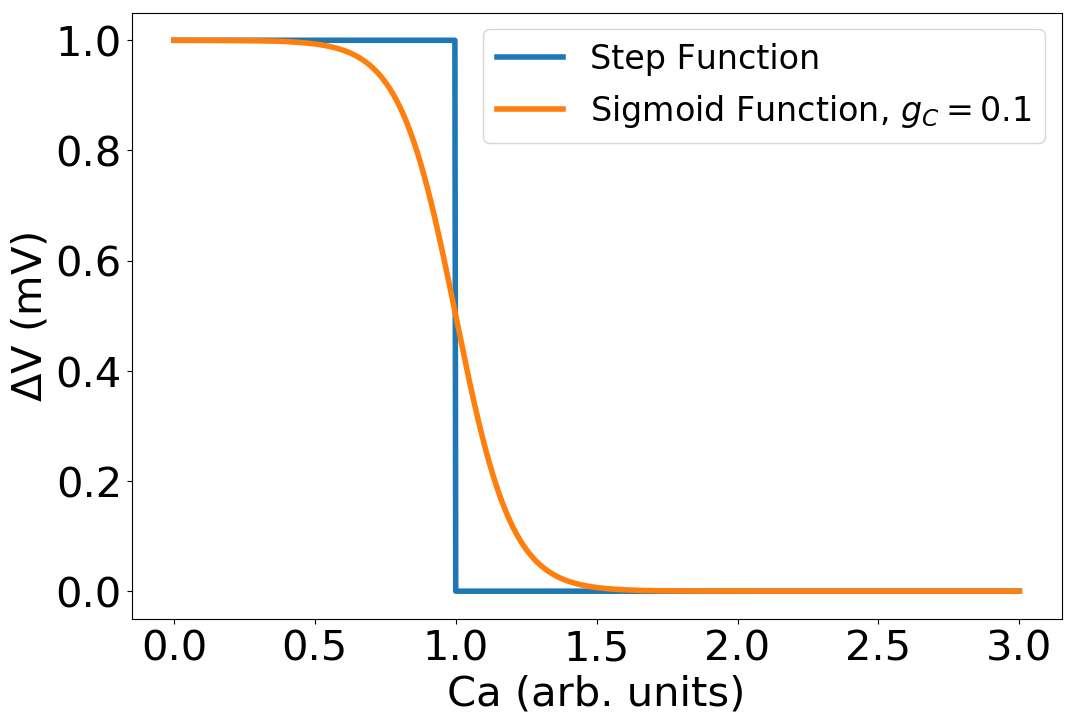
\includegraphics[width=65mm]{calcium_concentration_step.png}
    \caption{Left: Firing rate, P(V) as function of potential voltage in membrane V with V$^*$=-55mV. Right: Voltage increment $\Delta V$ as a function of action potential received by neuron with C$^*$=1.0 \cite{kcore_paper}.}
    \label{fig:step_figures}
\end{figure}

%In the simplest case, the basal firing rate and calcium concentration functions of the neuron can be set to have no offset from 0 (fig. INSERT FIGURE HERE).\\

We set $\dot{V} = \dot{C} = 0$ to solve these equations (\ref{eq:step_voltage_increment} and \ref{eq:step_calcium_increment}) for the fixed point regime, and treat each resulting case separately (Appendix \ref{appendix:mean_field_analysis}).\\

From solving these equations analytically (Appendix \ref{appendix:mean_field_analysis}), we observe three different possible forms of the solution (fig. \ref{fig:step_mean_field}). A quiescent fixed point (Q), where all neurons in the network cease their firing. Secondly, there is a possibility to observe a high activity fixed point (HA), where all the neurons are trapped in a firing state, but never return to the basal firing rate. Finally, given particular conditions, we observe stable oscillations (SO), wherein the neurons are constantly alternating between their maximum firing rate, and their basal rate.\\

\begin{figure}
  \centering
  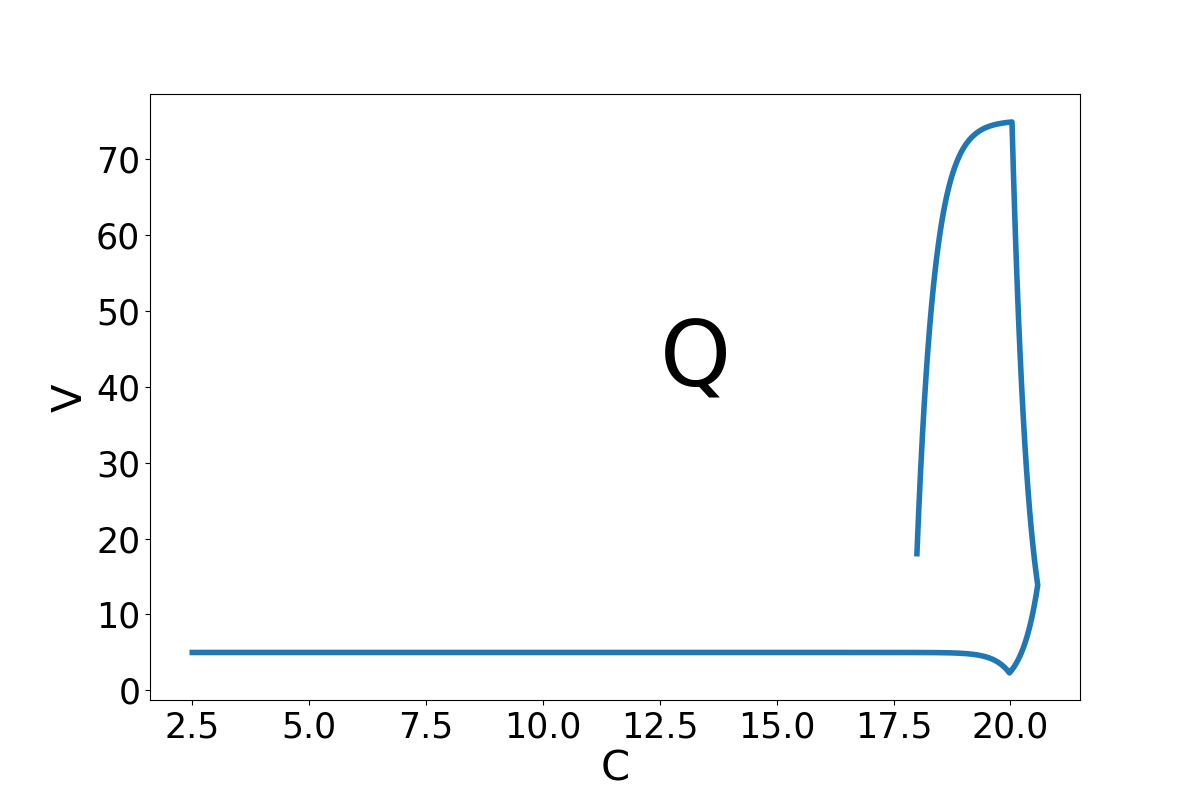
\includegraphics[width=50mm]{step_low.png}
  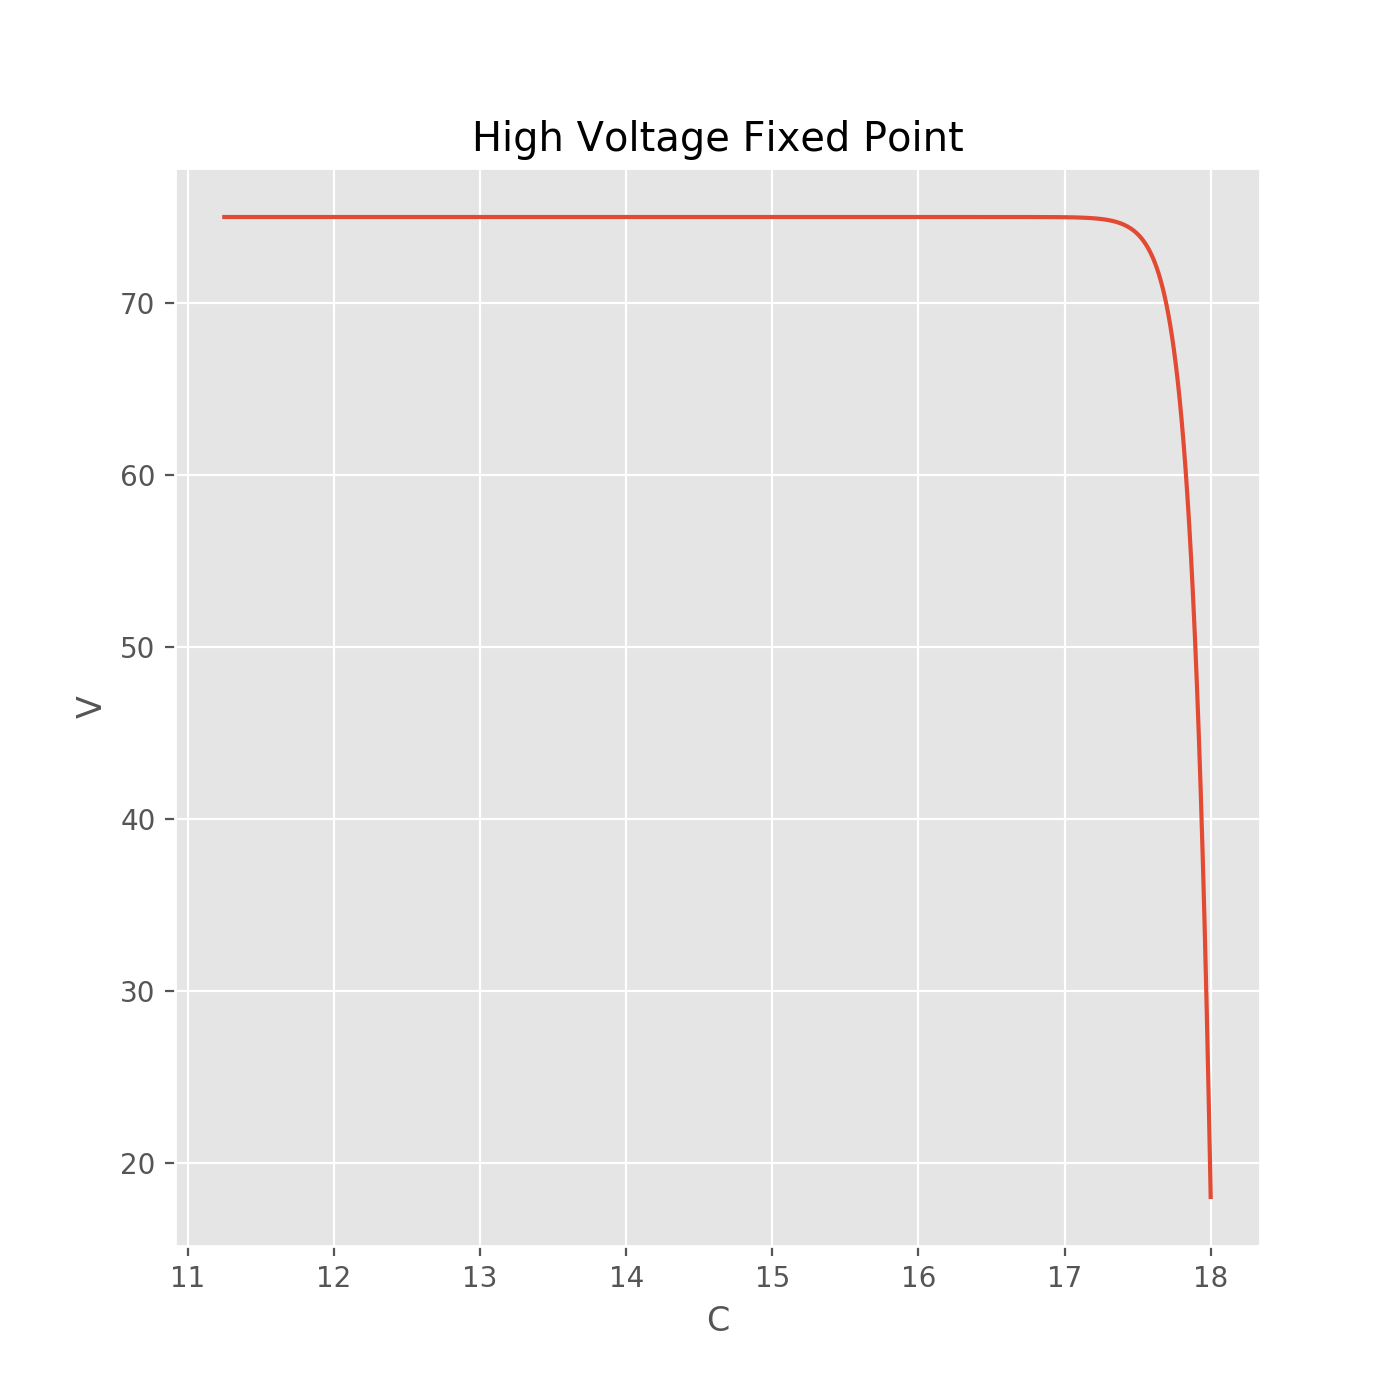
\includegraphics[width=50mm]{step_high.png}
  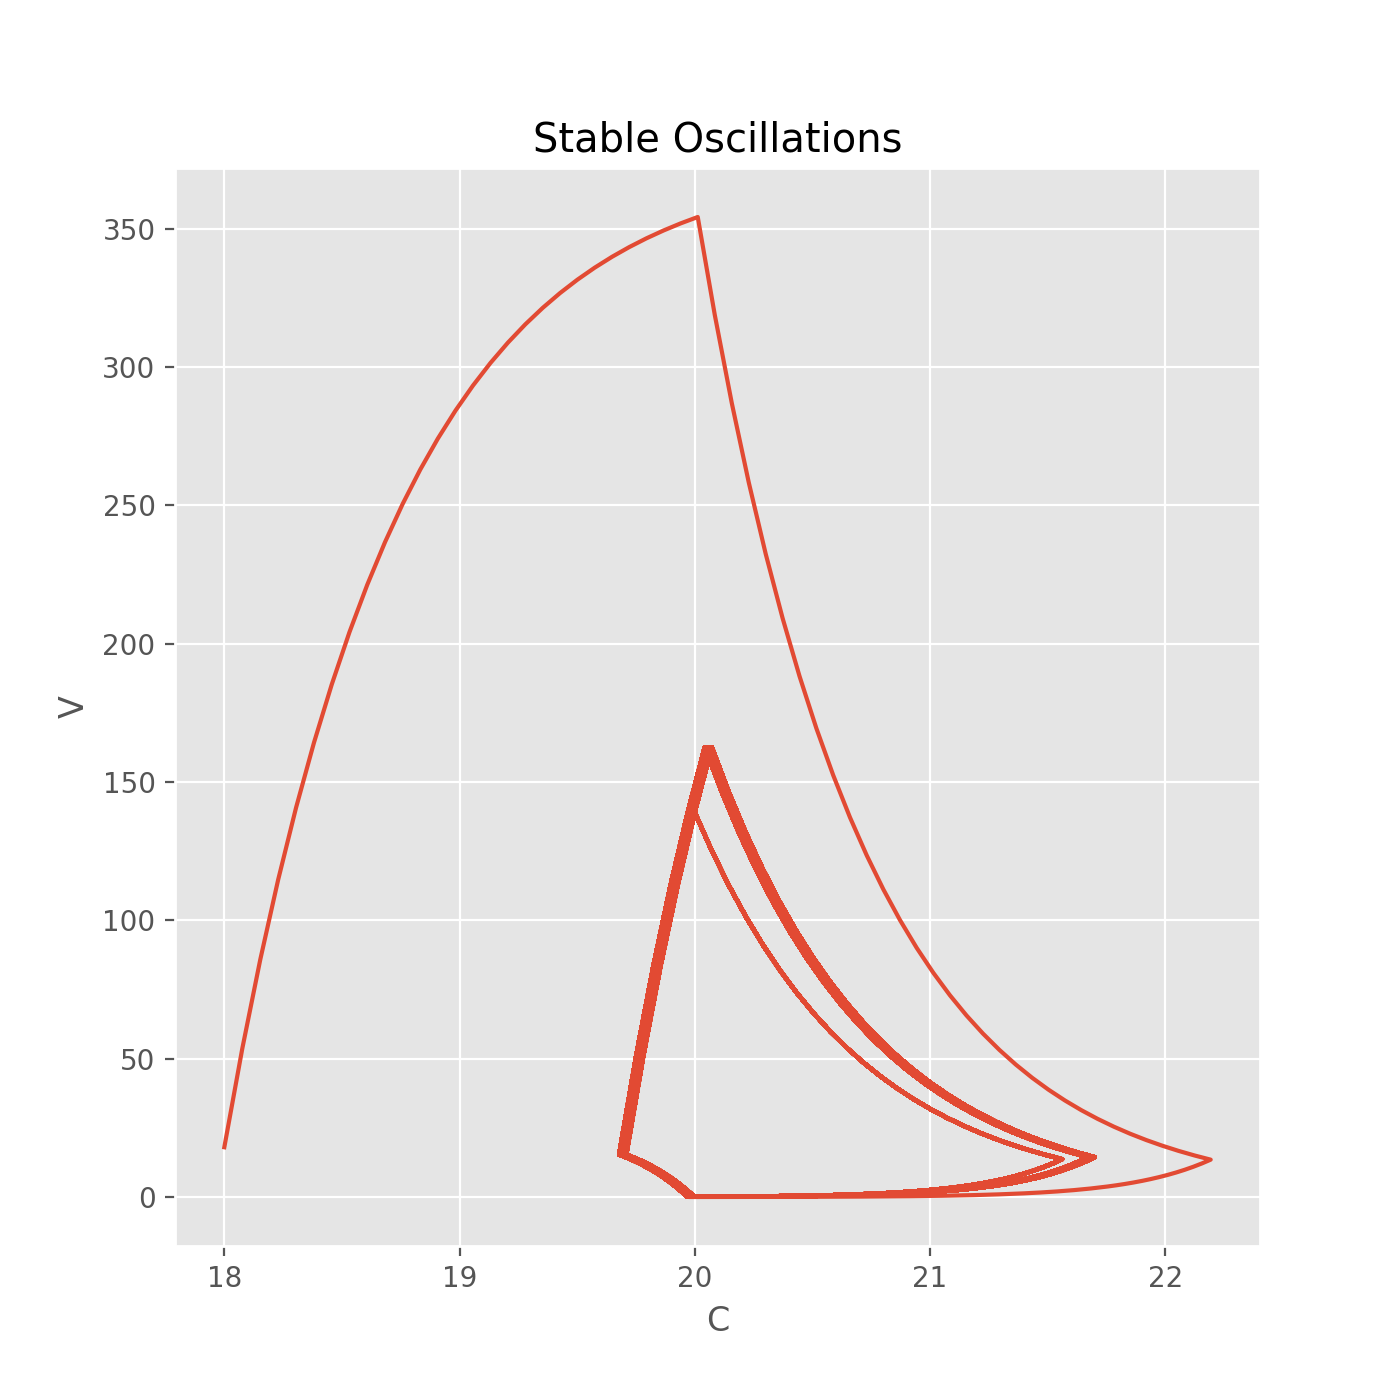
\includegraphics[width=50mm]{step_SO.png}
  \caption{(Left) Low voltage fixed point (Q), (Center) High voltage fixed point (HA), (Right) Stable Oscillations (S).}
  \label{fig:step_mean_field}
\end{figure}

We demonstrate the phase space of the possible solutions to equations \ref{eq:voltage_increment} and \ref{eq:calcium_increment} in the mean field limit in figure \ref{fig:mean_field_phase}. These results are somewhat similar to those of the mean field analysis by Schwab et al. \cite{kcore_paper}. As neurons are culled from the network at random, a relatively smooth phase boundary is observed between the SO and fixed point phases. The location of the triple point in the Ca$^{2+}$ phase diagram depends in part on the choice of $\Delta V$ used.

\begin{figure}
	\centering
    	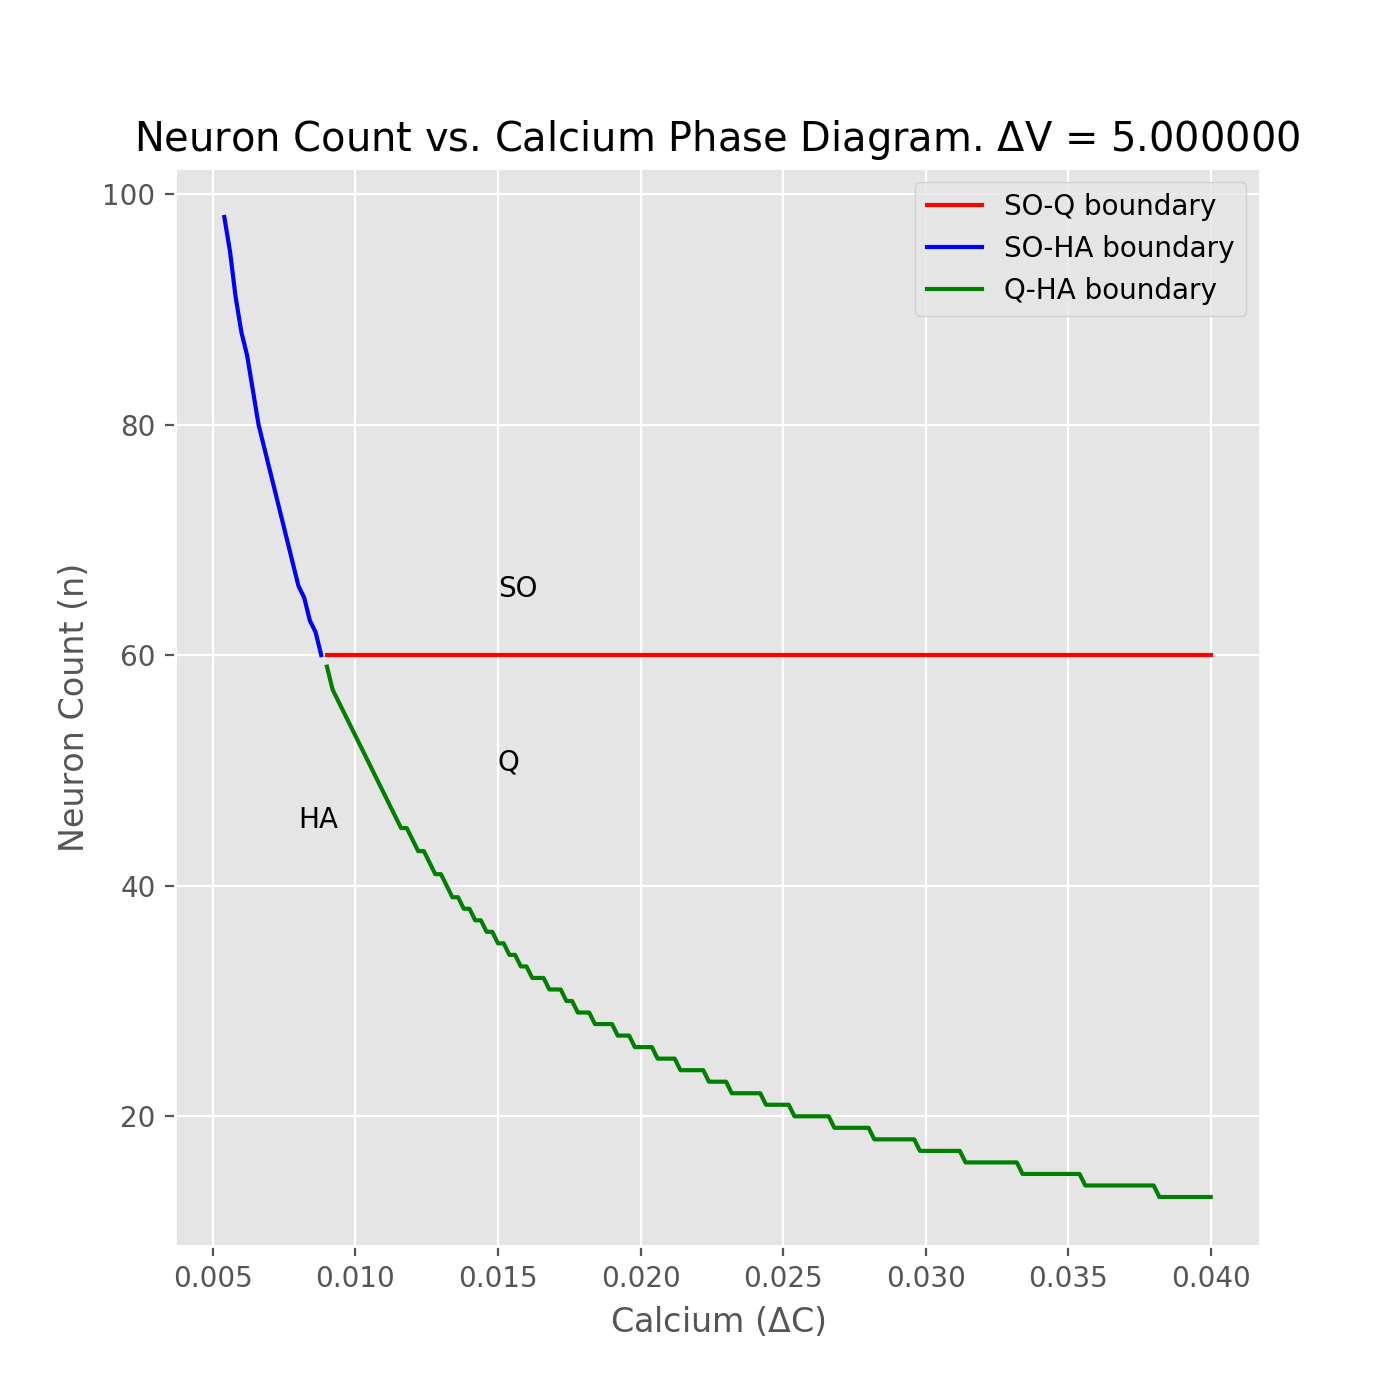
\includegraphics[width=50mm]{step_nC_phase.png}
        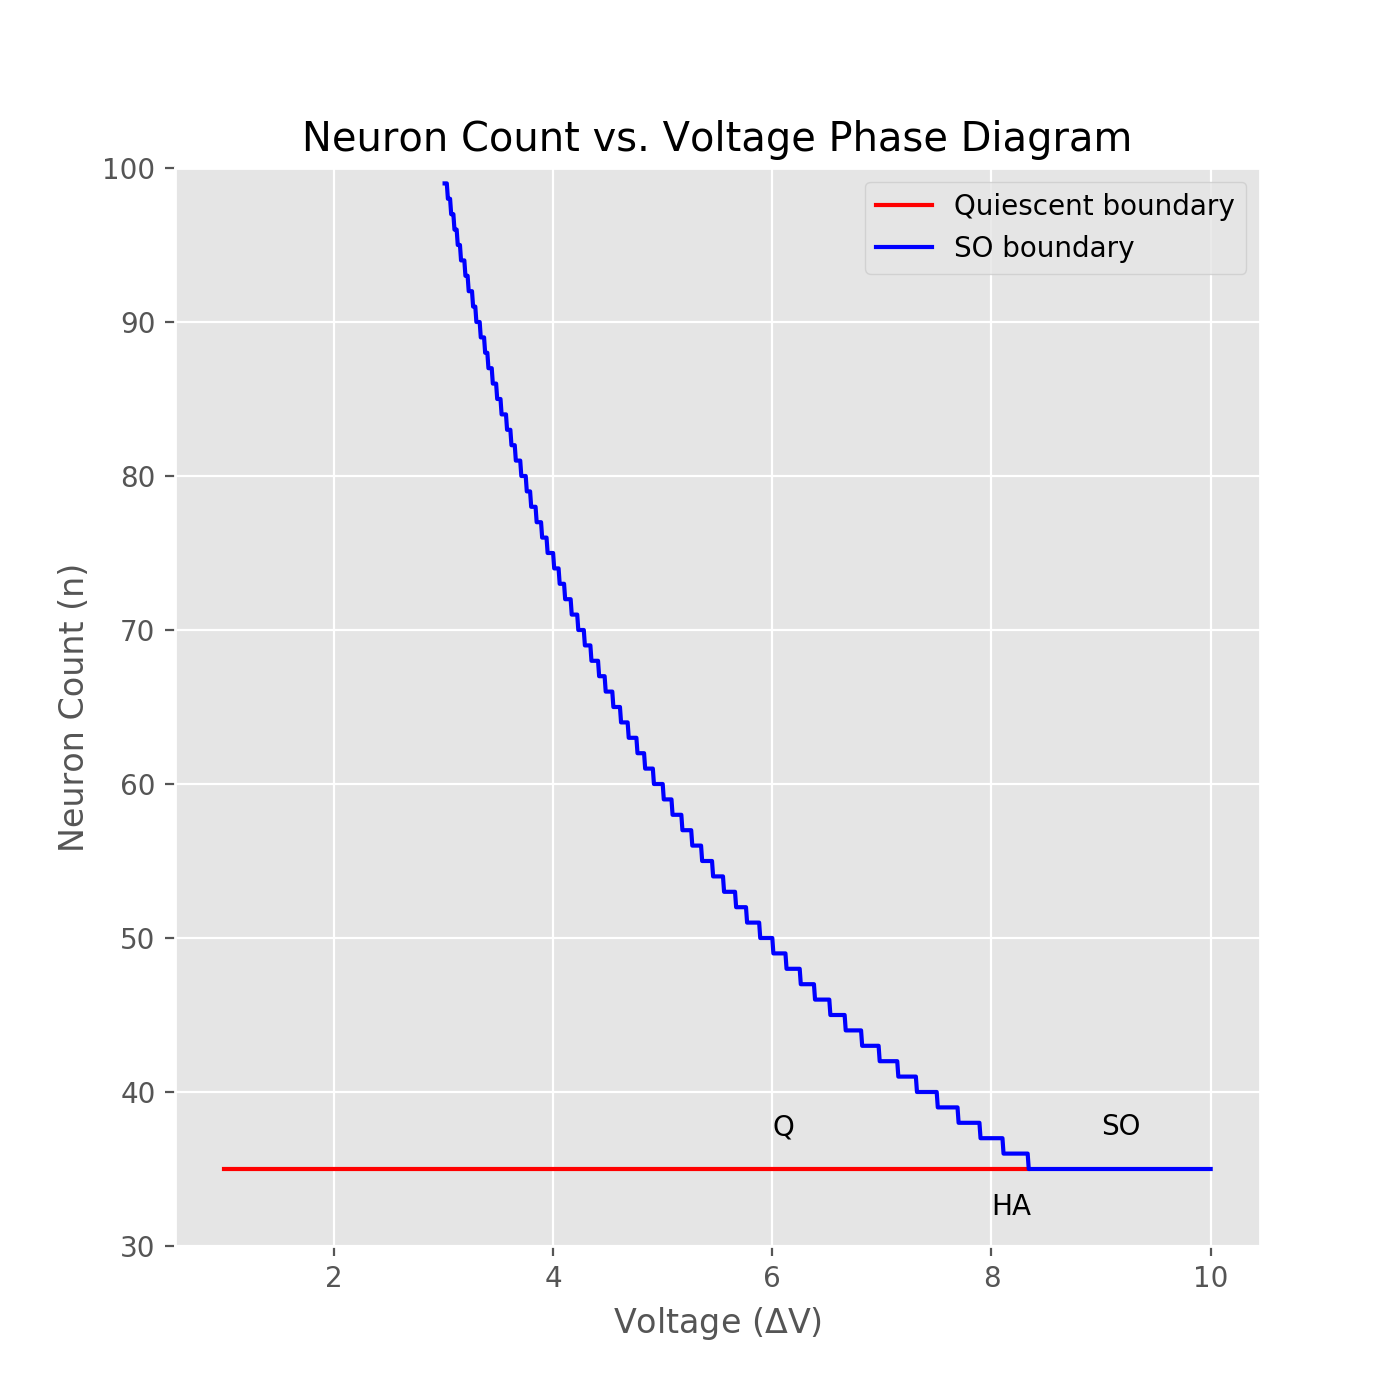
\includegraphics[width=50mm]{step_nV_phase.png}
    \caption{Left: Phase diagram in neuron count and Ca$^2+$ concentration of homogeneous N-neuron network. The horizontal axis represents the local Ca$2+$ ion concentration. Right: Phase diagram in neuron count and Voltage of homogeneous N-neuron network. The horizontal axis represents the maximum somatic voltage jump of a cell following an input pulse \cite{kcore_paper}.}
    \label{fig:mean_field_phase}
\end{figure}

\section{Analysis Applied to Heterogeneously Connected Network}
To simulate the heterogeneously connected system, an Erdos-Renyi network is generated by populating an adjacency matrix with 1's and 0's according to a specified probability value. We consider the simplest possible model that allows us to recover information about the largest k k-core in the network in equations \ref{eq:simple_model_firing} and \ref{eq:simple_model_calcium}. Here, $r$ is the firing rate of the neurons as a function of voltage.

\begin{equation}
\dot{V_i} = -\frac{1}{\tau _V}V_i + \sum _{i=1} ^{N} M_{ij}\Delta V(C_i) r(V_j)
\label{eq:simple_model_firing}
\end{equation}

\begin{equation}
\dot{C_i} = -\frac{1}{\tau _C} C_i + \sum _{i=1} ^{N} M_{ij}\Delta C r(V_j)
\label{eq:simple_model_calcium}
\end{equation}

%Include solving for this analytically in the appendix
Solving for $\dot{V_i} = 0$ and $\dot{C_i} = 0$, we arrive at an expression that can be used to find the $k$ value of the largest $k$-core in the network (eq. ).

\begin{equation}
k=\frac{V^*}{\tau _V \Delta V_{\text{min}} r_{\text{max}}}
\label{eq:kcore_predictor}
\end{equation}

%This is the punchline so deliver it well
We use equation \ref{eq:kcore_predictor} as a $k$-core predictor. Effectively, given four parameters of the network and no adjacency matrix, we are able to determine the value of $k$ for the largest $k$-core in the network. Moreover, as neurons are randomly culled from the network, or the value of $\Delta V$ is adjusted to explore the phase space, the actual value of $k$ can be computed exactly. The predicted values of $k$ from equation \ref{eq:kcore_predictor} are found to correspond exactly to the true $k$ value of the largest $k$-core of the network as neurons are culled from the network at random (fig: \ref{fig:kcore_exact_vs_predict}).

\begin{figure}[ht]
	\centering
    	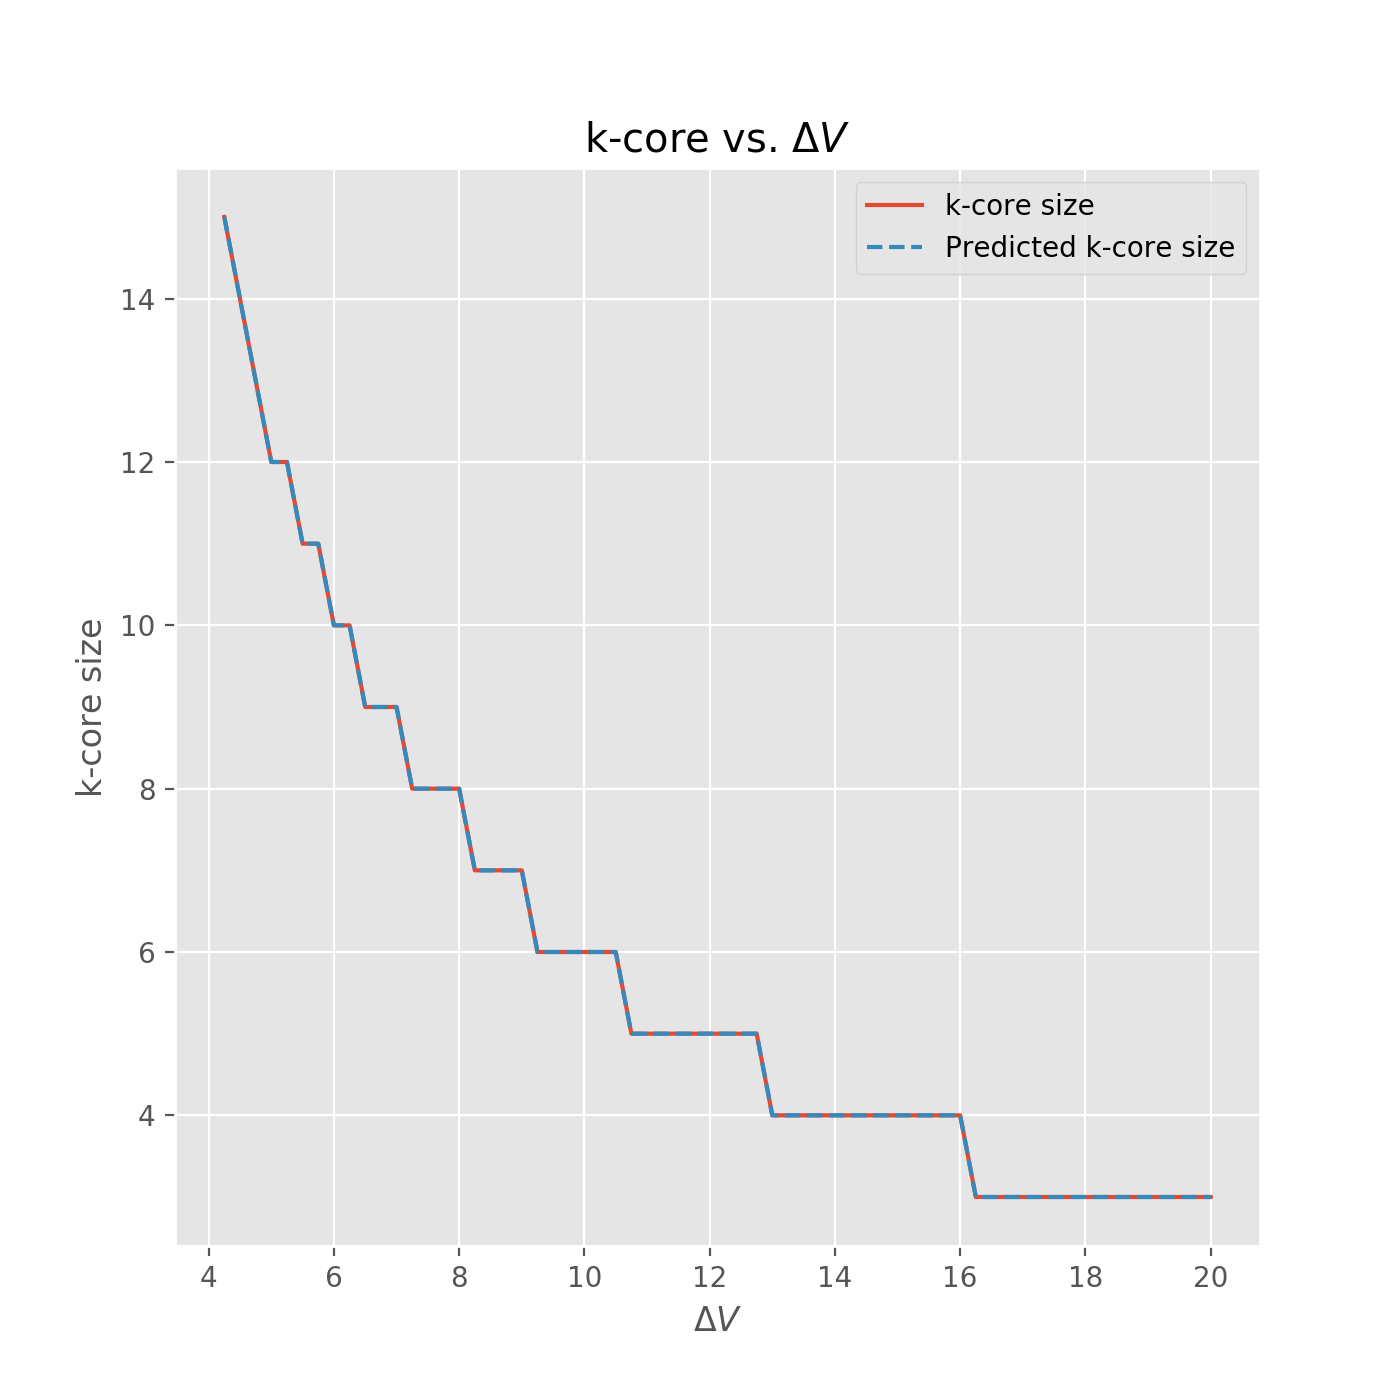
\includegraphics[width = 90mm]{kcore_exact_vs_predict.png}\\
    \caption{Demonstration of the exact correspondence between the predicted $k$ value and the true $k$ value of the largest $k$-core in the network.}
    \label{fig:kcore_exact_vs_predict}
\end{figure}

\begin{thebibliography}{9}
\bibitem{kcore_paper}
Schwab, D. J., Bruinsma, R. F., Feldman, J. L., $\&$ Levine, A. J. (2010). Rhythmogenic neuronal networks, emergent leaders, and k-cores.
\textit{Physical Review. E, Statistical, Nonlinear, and Soft Matter Physics}, 82(5 Pt 1), 051911.

\bibitem{koch}
Koch, C. Biophysics of Computation. Oxford University Press; New York: 1999.

\bibitem{preBotzinger_paper}
Smith, J. C., Ellenberger, H. H., Ballanyi, K., Richter, D. W., $\&$ Feldman, J. L. (1991). Pre-Bötzinger Complex: A Brainstem Region That May Generate Respiratory Rhythm in Mammals. \textit{Science} (New York, N.Y.), 254(5032), 726–729.

\bibitem{feldman_del_negro}
Feldman, J. L., $\&$ Del Negro, C. A. (2006). Looking for inspiration: new perspectives on respiratory rhythm. \textit{Nature Reviews}. Neuroscience, 7(3), 232.

\bibitem{network_structure_minimum_degree}
Siedman, S. (1983). Network Structure and Minimum Degree. \textit{Social Networks}.

\bibitem{preBotzinger_anatomy}
Thoby-Brisson, M., $\&$ Greer, J. J. (2008). Anatomical and functional development of the pre-Bötzinger complex in prenatal rodents. \textit{Journal of Applied Psychology}. American Physiological Society.

\end{thebibliography}
\newpage
%TODO: Label Appendices for reference
\begin{appendices}
\section{Mean Field Analysis}
\label{appendix:mean_field_analysis}
\subsection*{Case I: $V < V^*, C > C^*$}
Solving for $V$ and $C$, we get:
\begin{equation}
V = n\tau _v \Delta V_1 r_0
\end{equation}
\begin{equation}
C = n\tau _c \Delta C r_0
\end{equation}

The resulting phase diagram is defined as having a low voltage fixed point. [TODO: Explain what classifies it as "low voltage" and include Image]

\subsection*{Case II: $V < V^*, C < C^*$}
$\Delta V$ goes to 0 so:
\begin{equation}
V = n\tau _v \Delta V_0 r_0
\end{equation}
\begin{equation}
C = n\tau _c \Delta C r_0
\end{equation}

\subsection*{Case III: $V > V^*, C > C^*$}
$\Delta V$ goes to 0 so:
\begin{equation}
V = n\tau _v \Delta V_0 r_1
\end{equation}
\begin{equation}
C = n\tau _c \Delta C r_1
\end{equation}

\subsection*{Case IV: $V > V^*, C < C^*$}
\begin{equation}
V = n\tau_v \Delta V_1 r_1
\end{equation}
\begin{equation}
C = n\tau_c \Delta C r_1
\end{equation}

The resulting phase diagram is defined as having a high voltage fixed point. [TODO: Explain what classifies it as "high voltage" and include Image]

Interestingly, there exists a phase diagram for stable oscillations given the following restrictions on the parameters $V^*$ and $C^*$:

\begin{equation}
n\tau _v \Delta V_0 r_1 < V^* < n\tau _v \Delta V_1 r_0
\end{equation}
\begin{equation}
n\tau _c \Delta C r_0 < C^* < n\tau_c \Delta C r_1
\end{equation}

\newpage
\section{Network Diagrams}
\label{appendix:network_diagrams}
\begin{figure}[!htb]
	\centering
  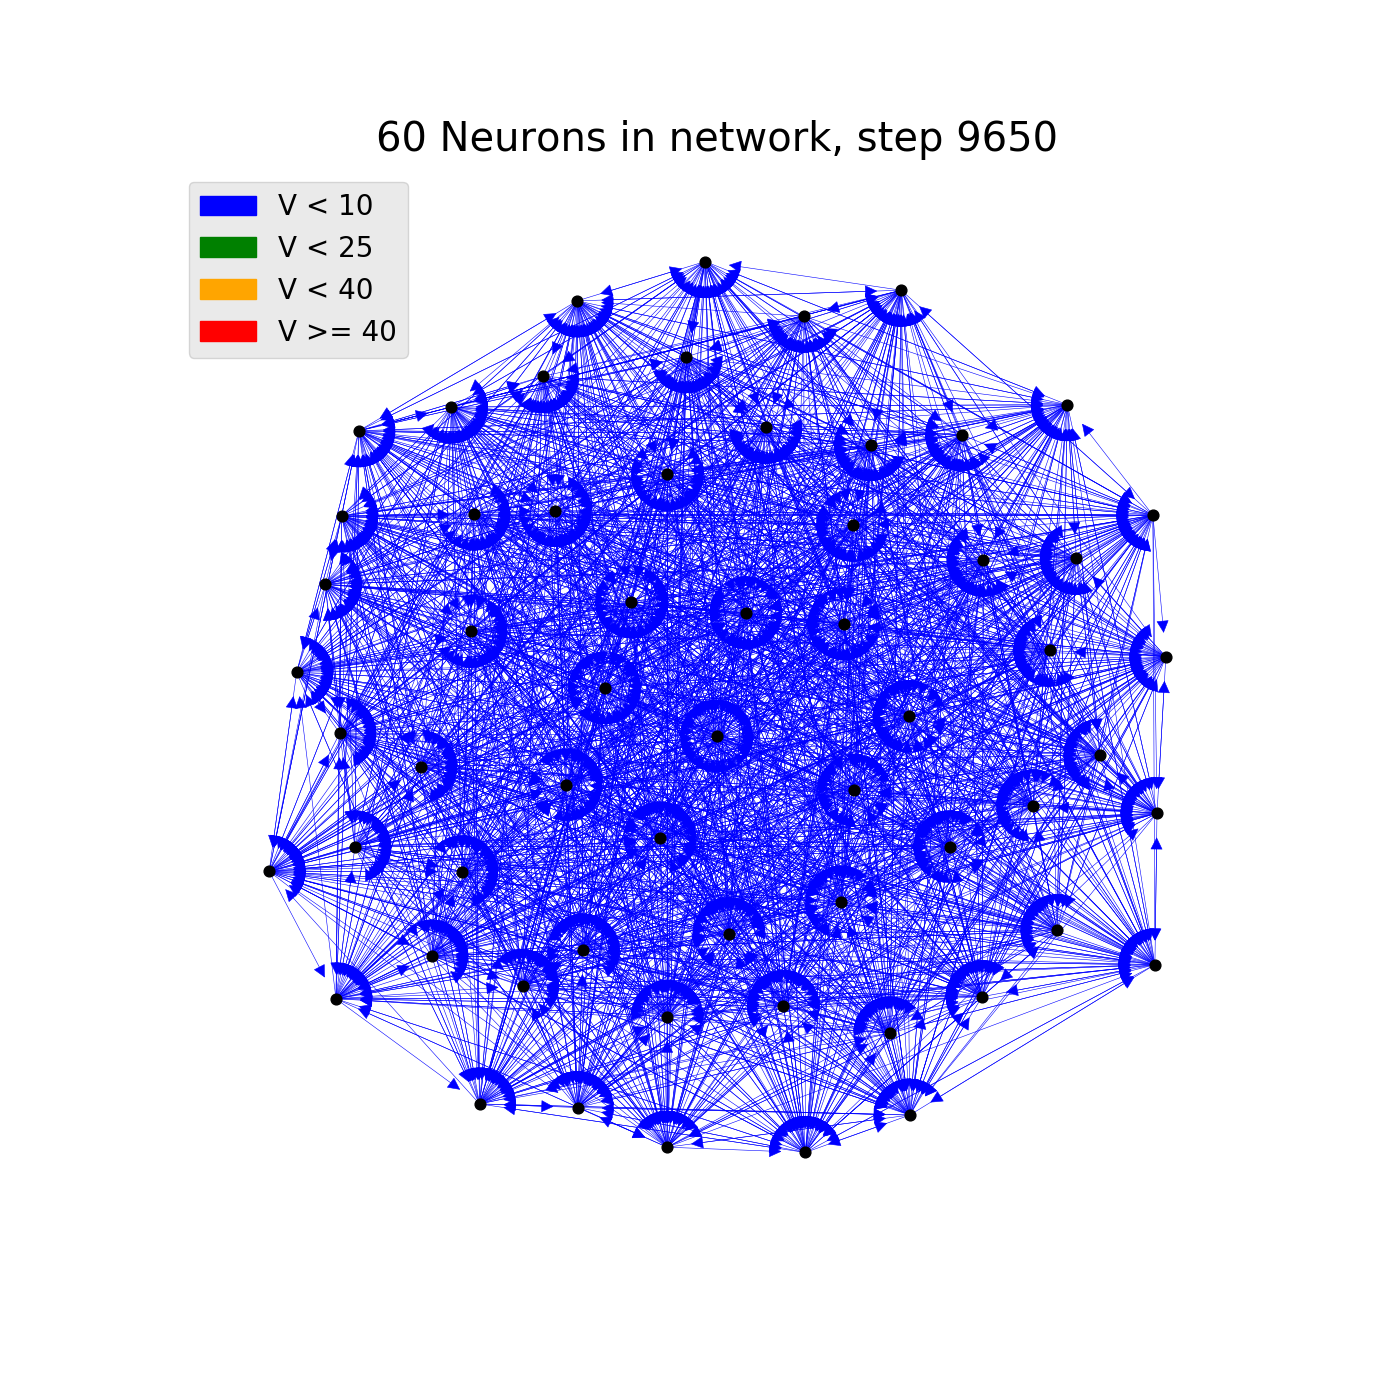
\includegraphics[width=40mm]{neuron_connectivity_at_step_9650}
  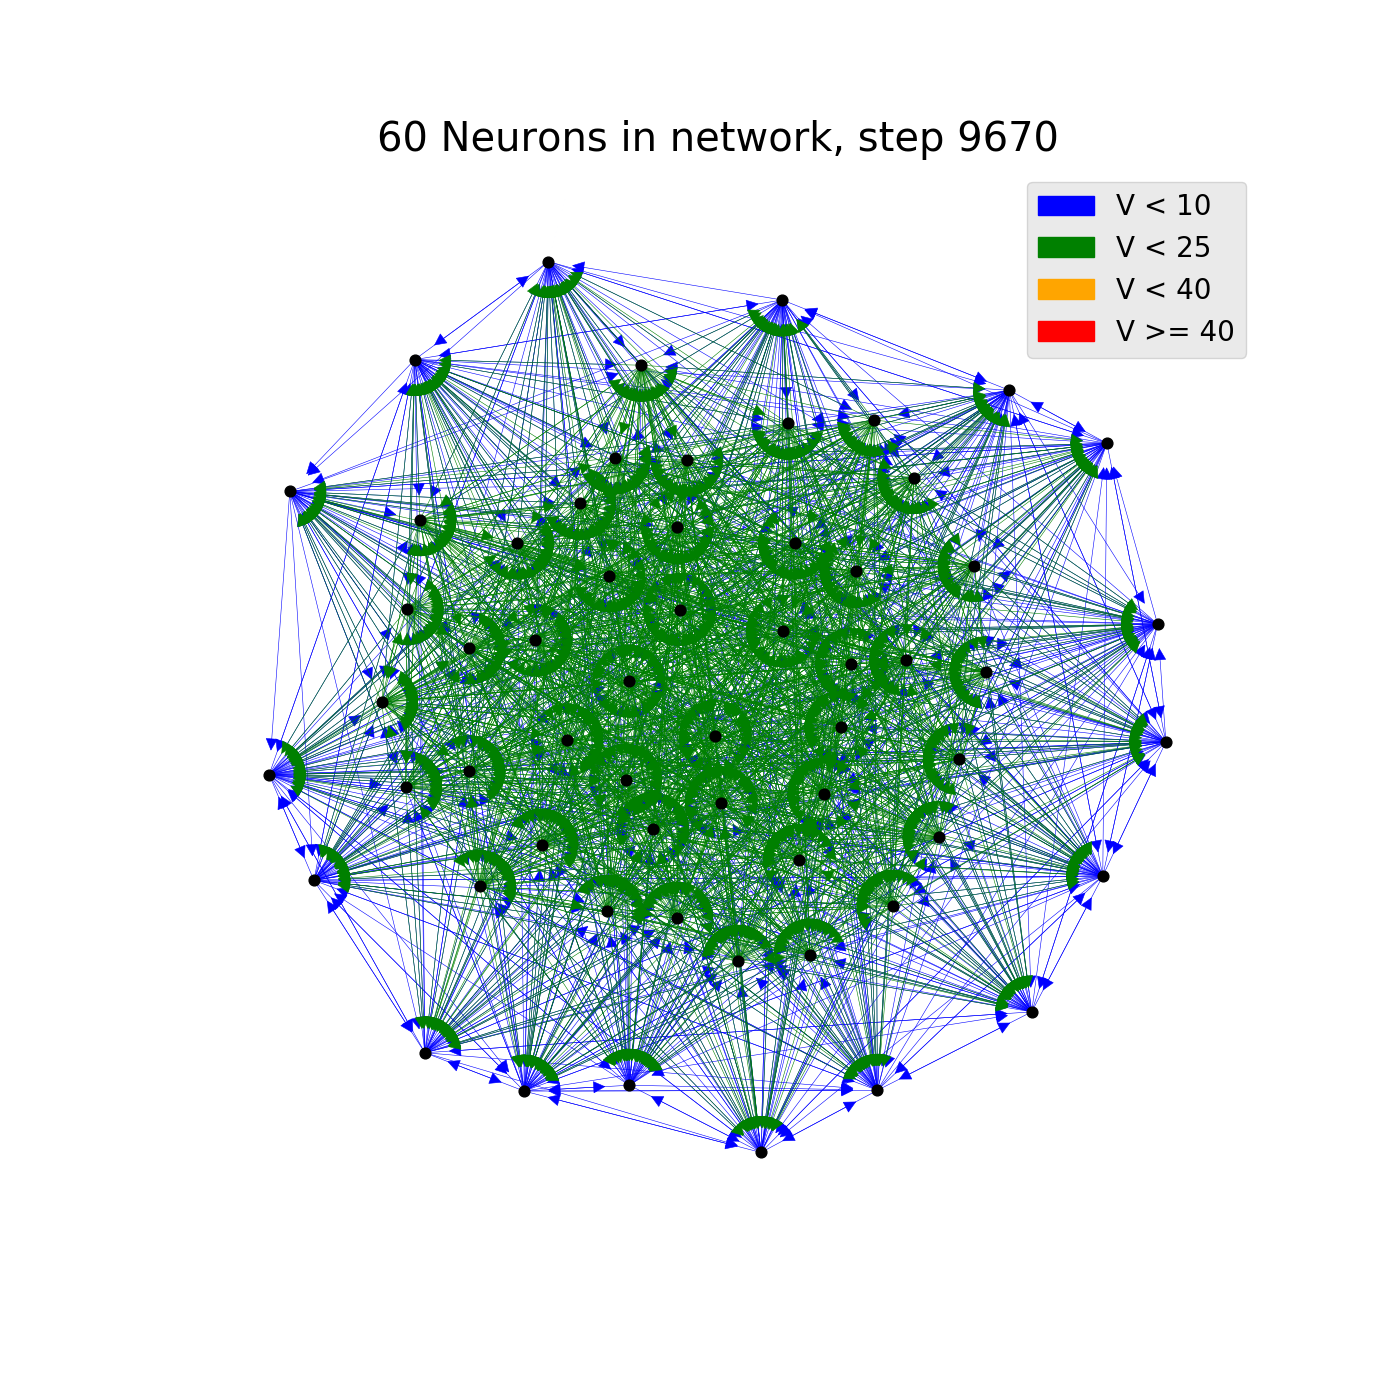
\includegraphics[width=40mm]{neuron_connectivity_at_step_9670}
  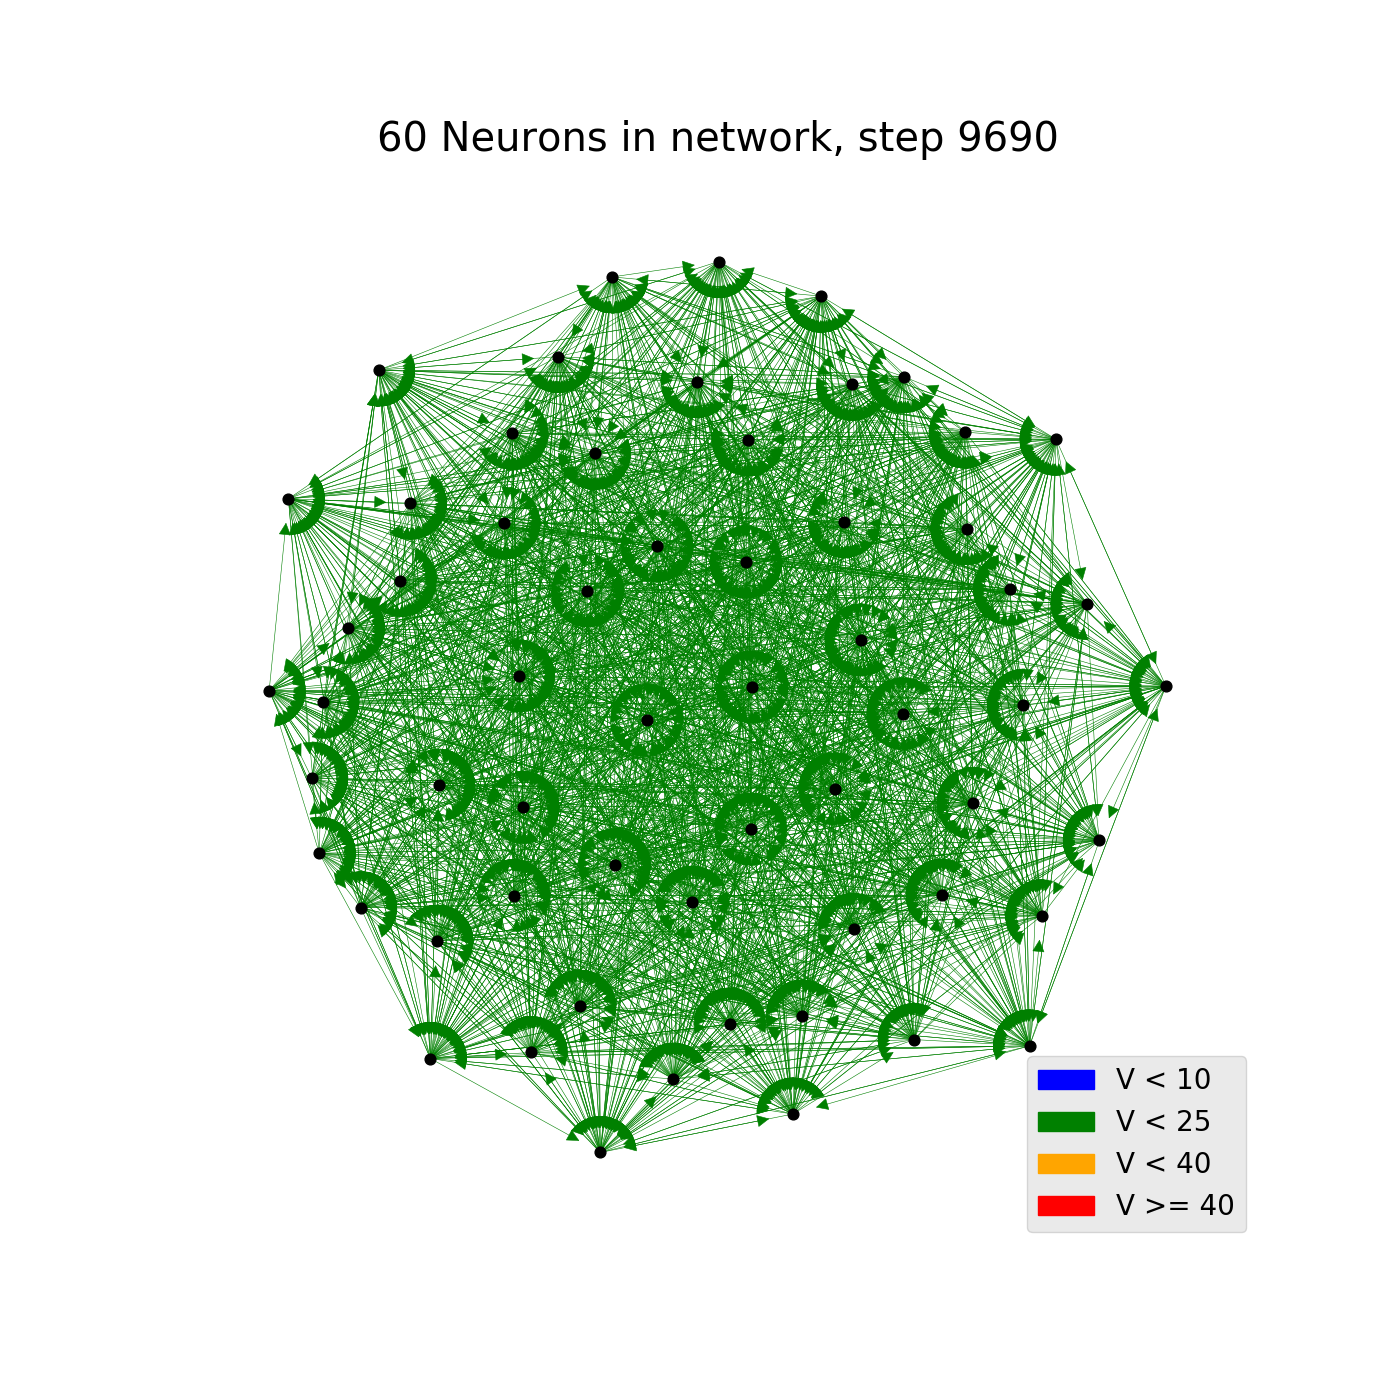
\includegraphics[width=40mm]{neuron_connectivity_at_step_9690}
  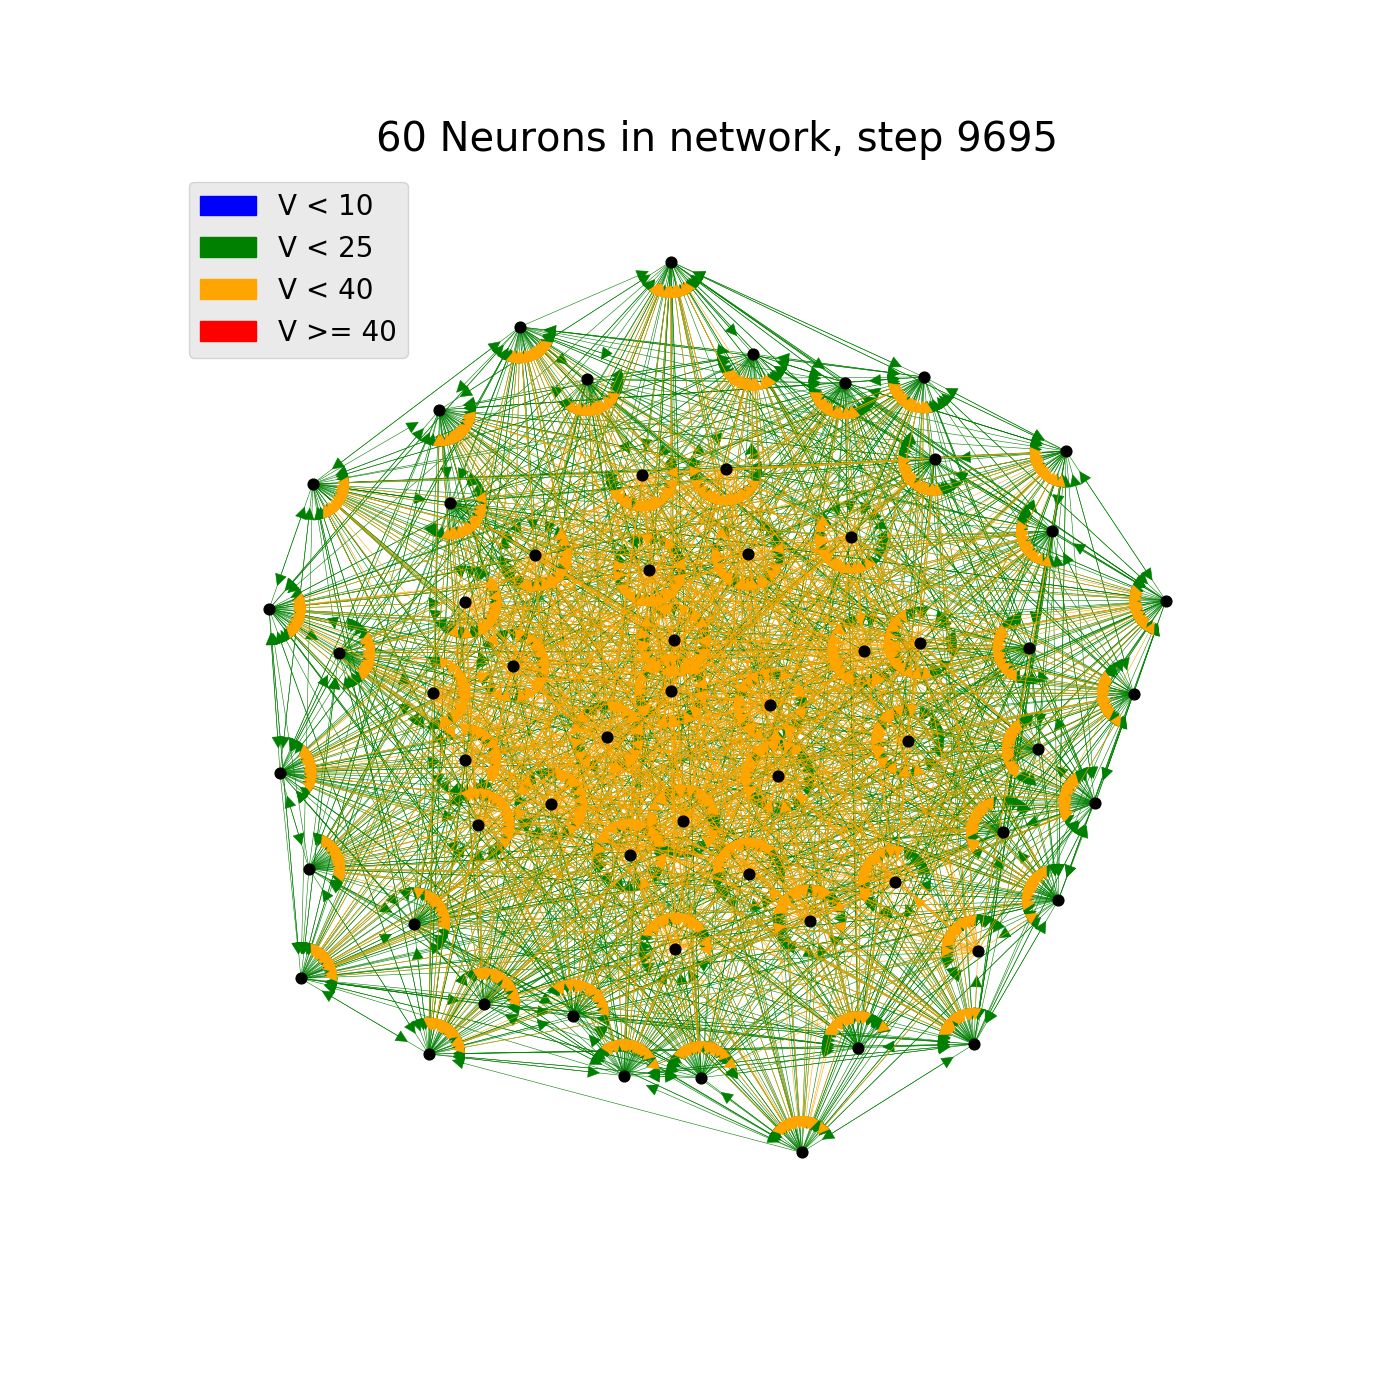
\includegraphics[width=40mm]{neuron_connectivity_at_step_9695}\\
  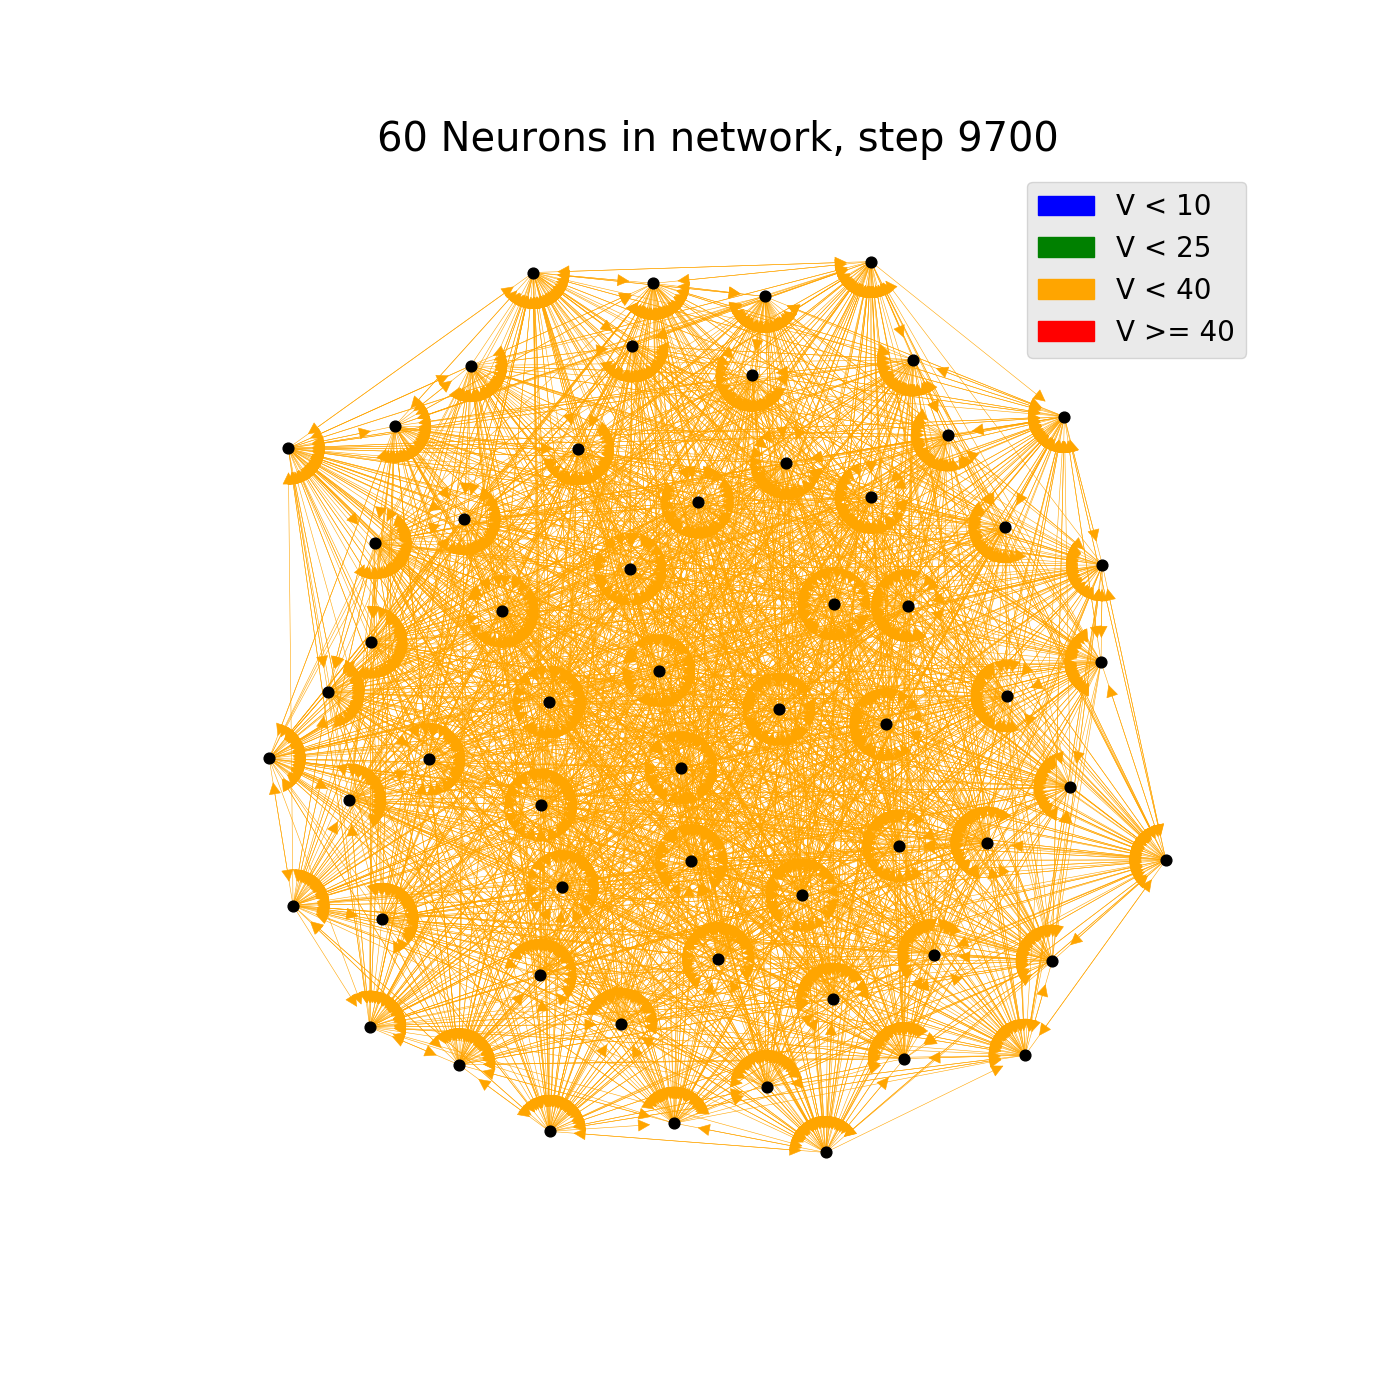
\includegraphics[width=40mm]{neuron_connectivity_at_step_9700}
  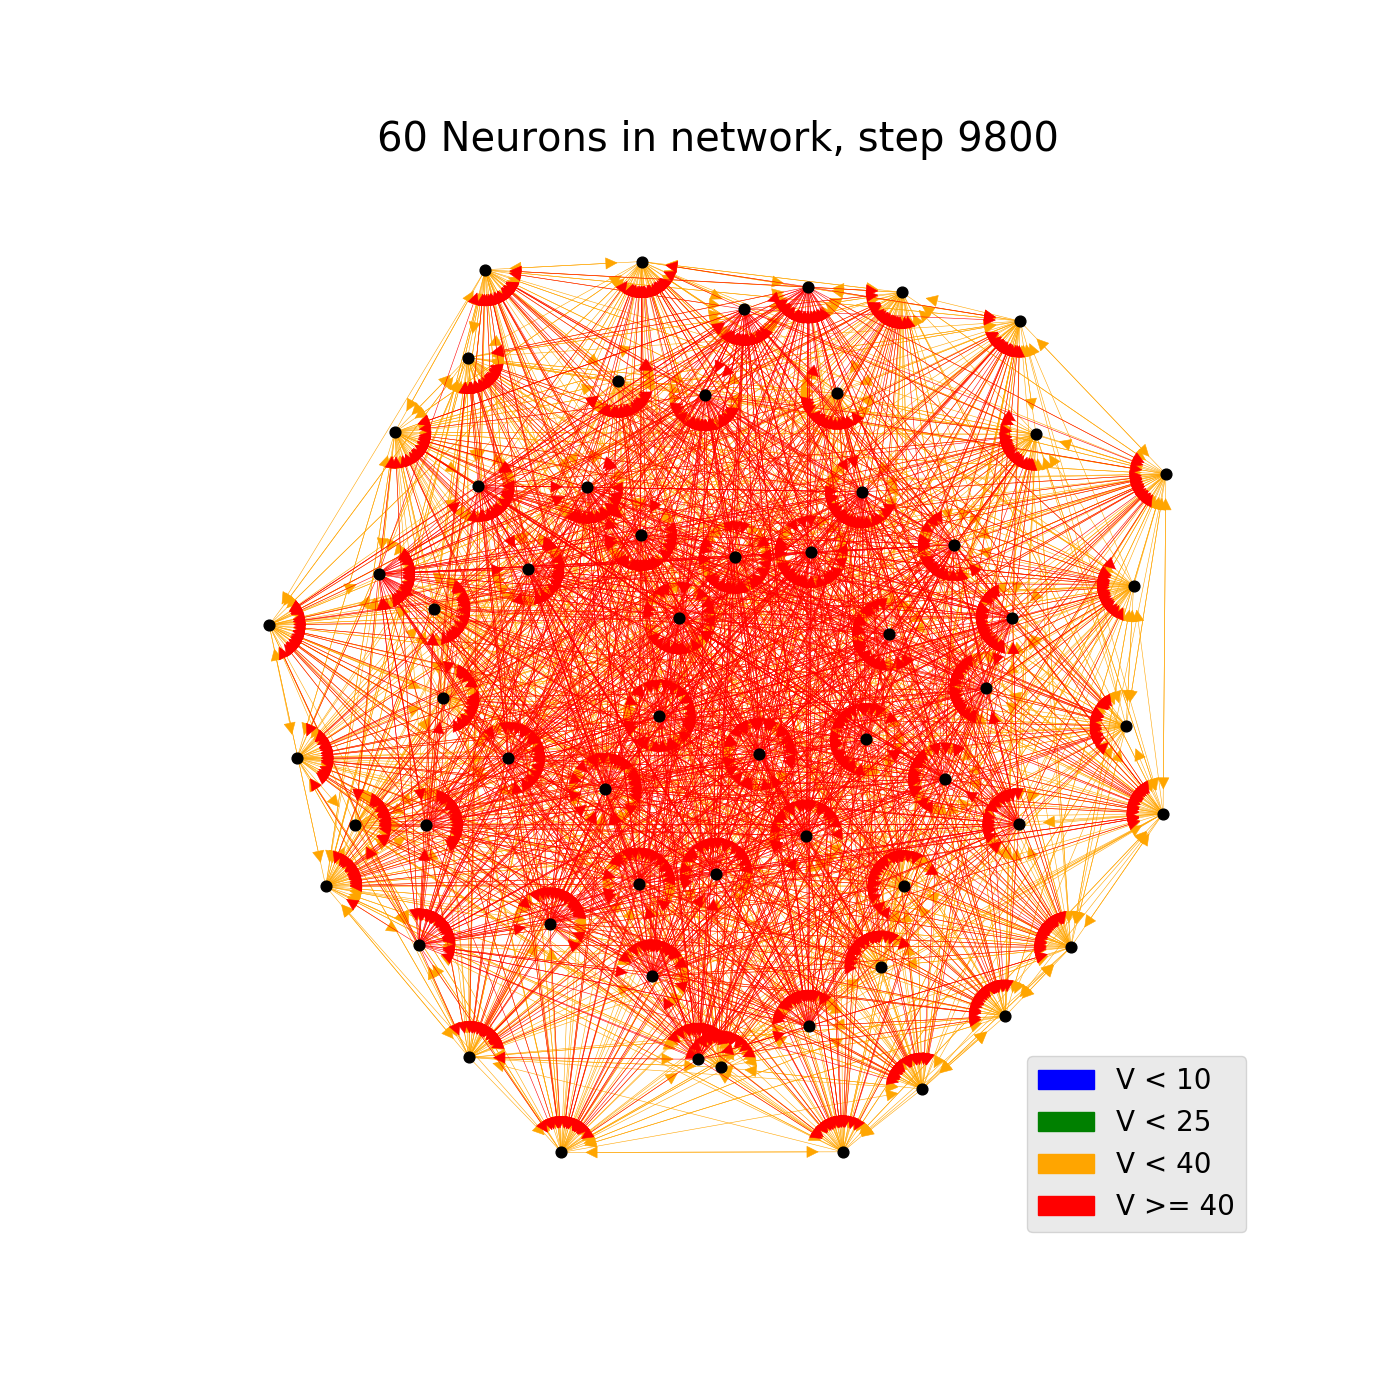
\includegraphics[width=40mm]{neuron_connectivity_at_step_9800}
  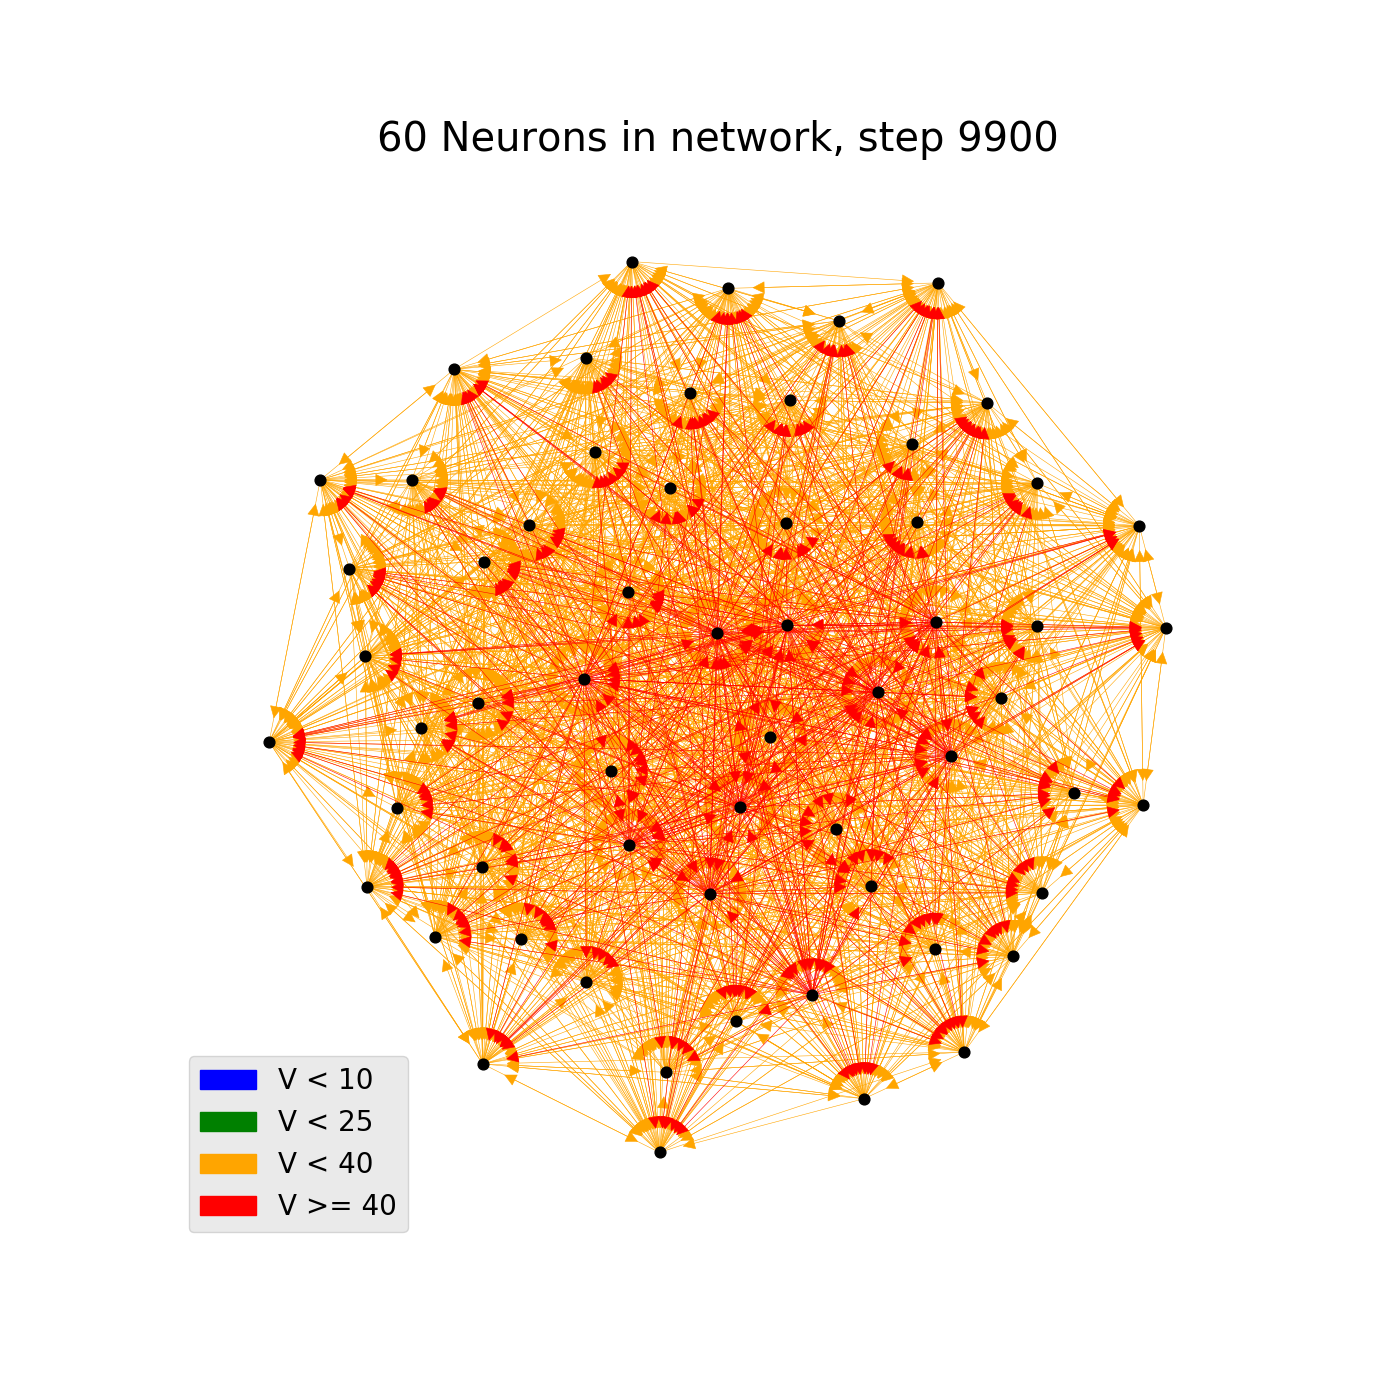
\includegraphics[width=40mm]{neuron_connectivity_at_step_9900}
  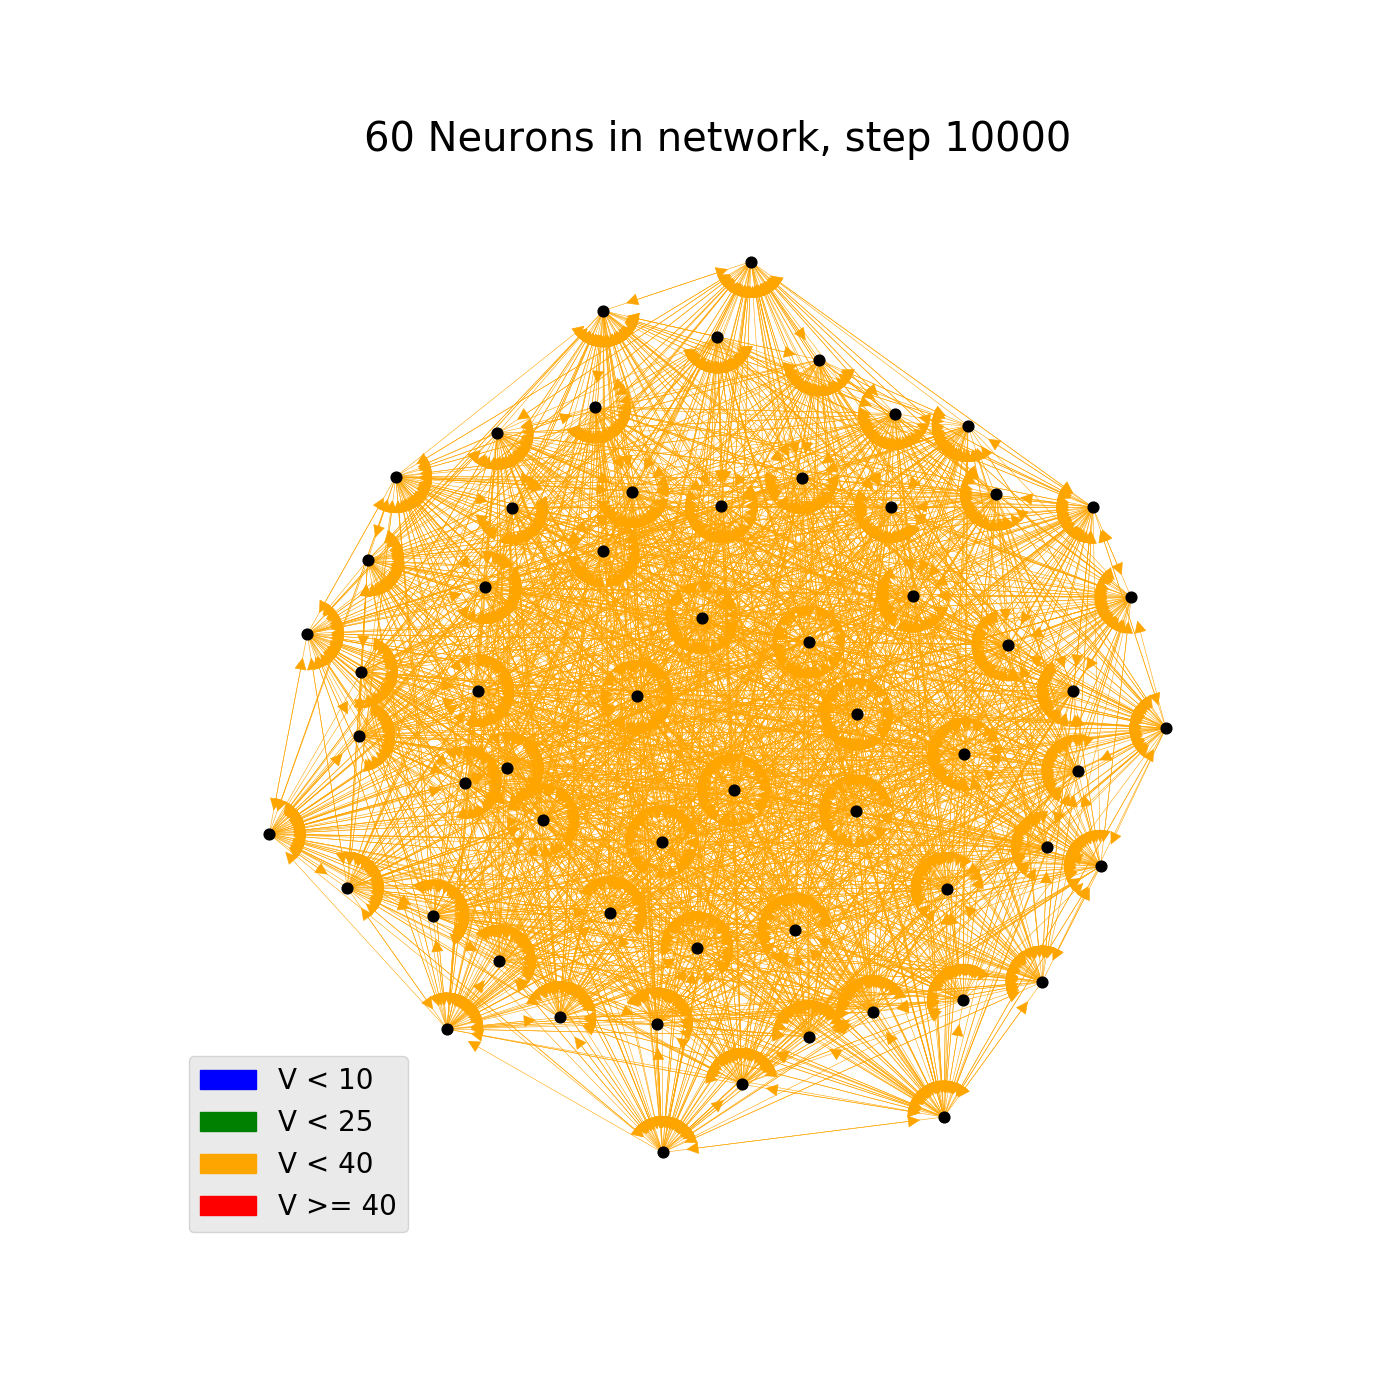
\includegraphics[width=40mm]{neuron_connectivity_at_step_10000}\\
  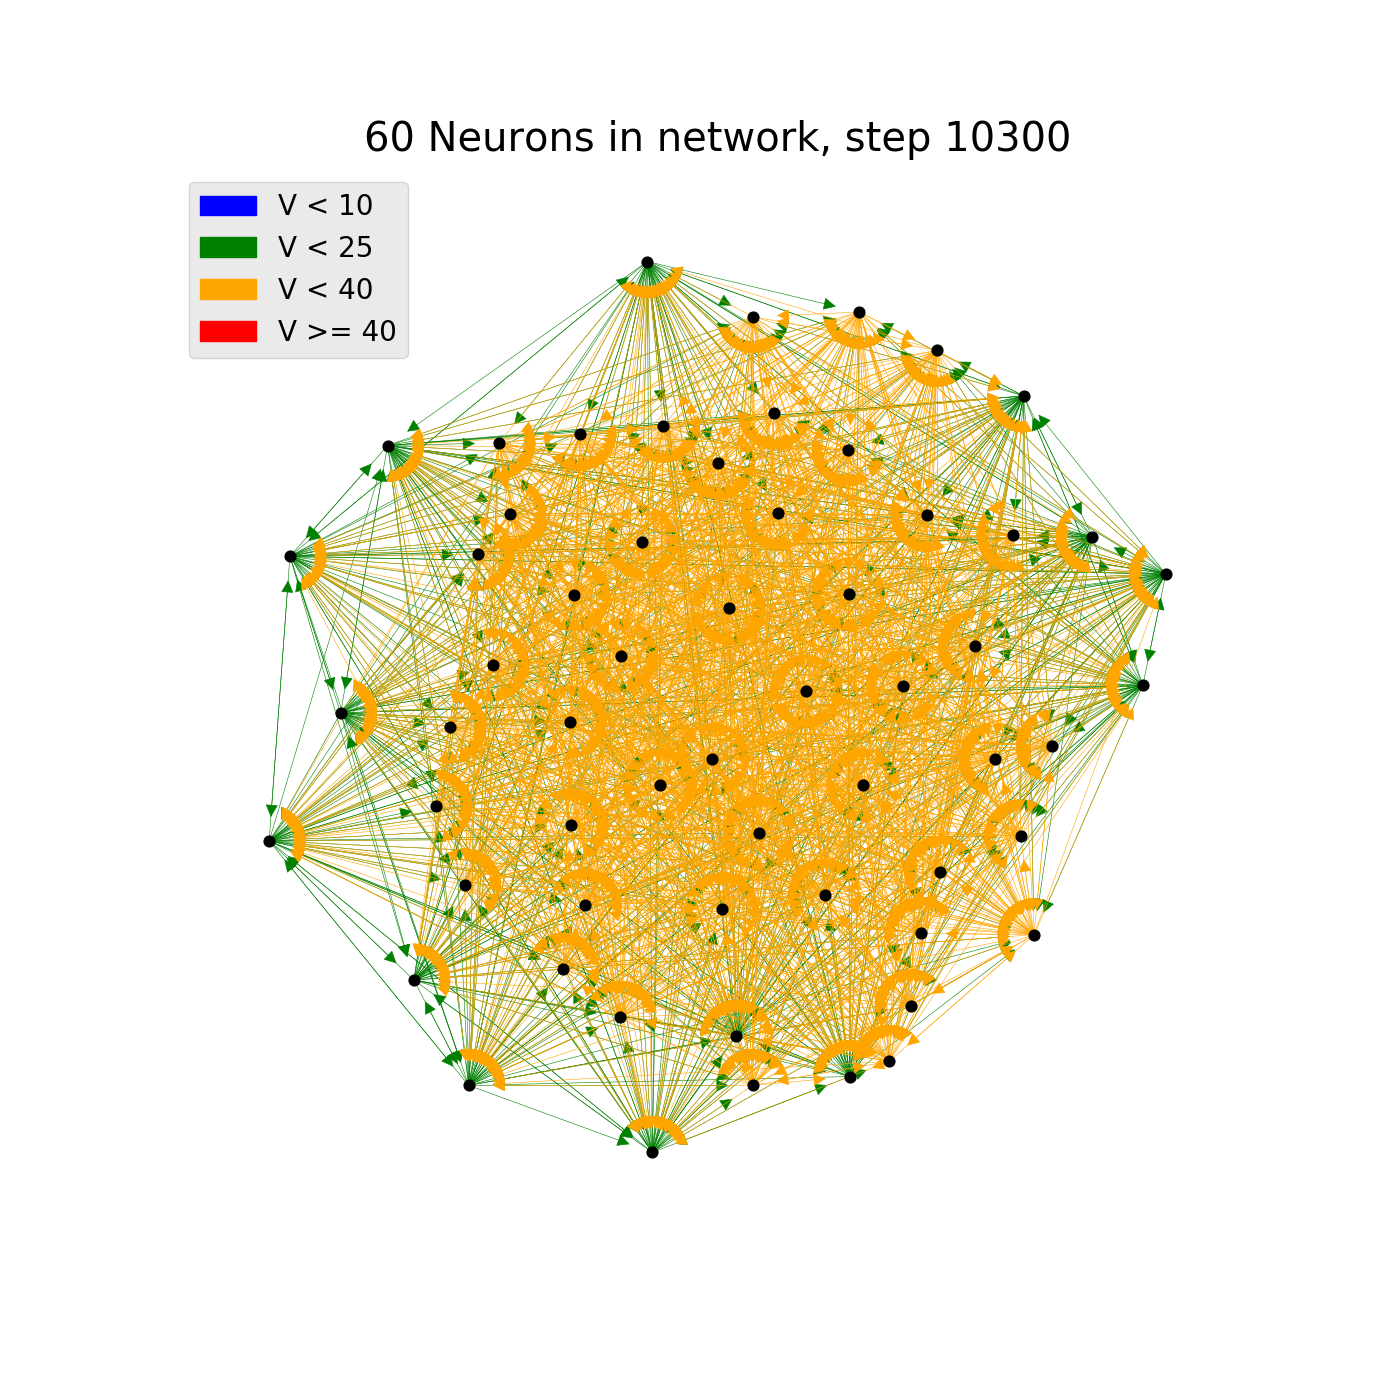
\includegraphics[width=40mm]{neuron_connectivity_at_step_10300}
  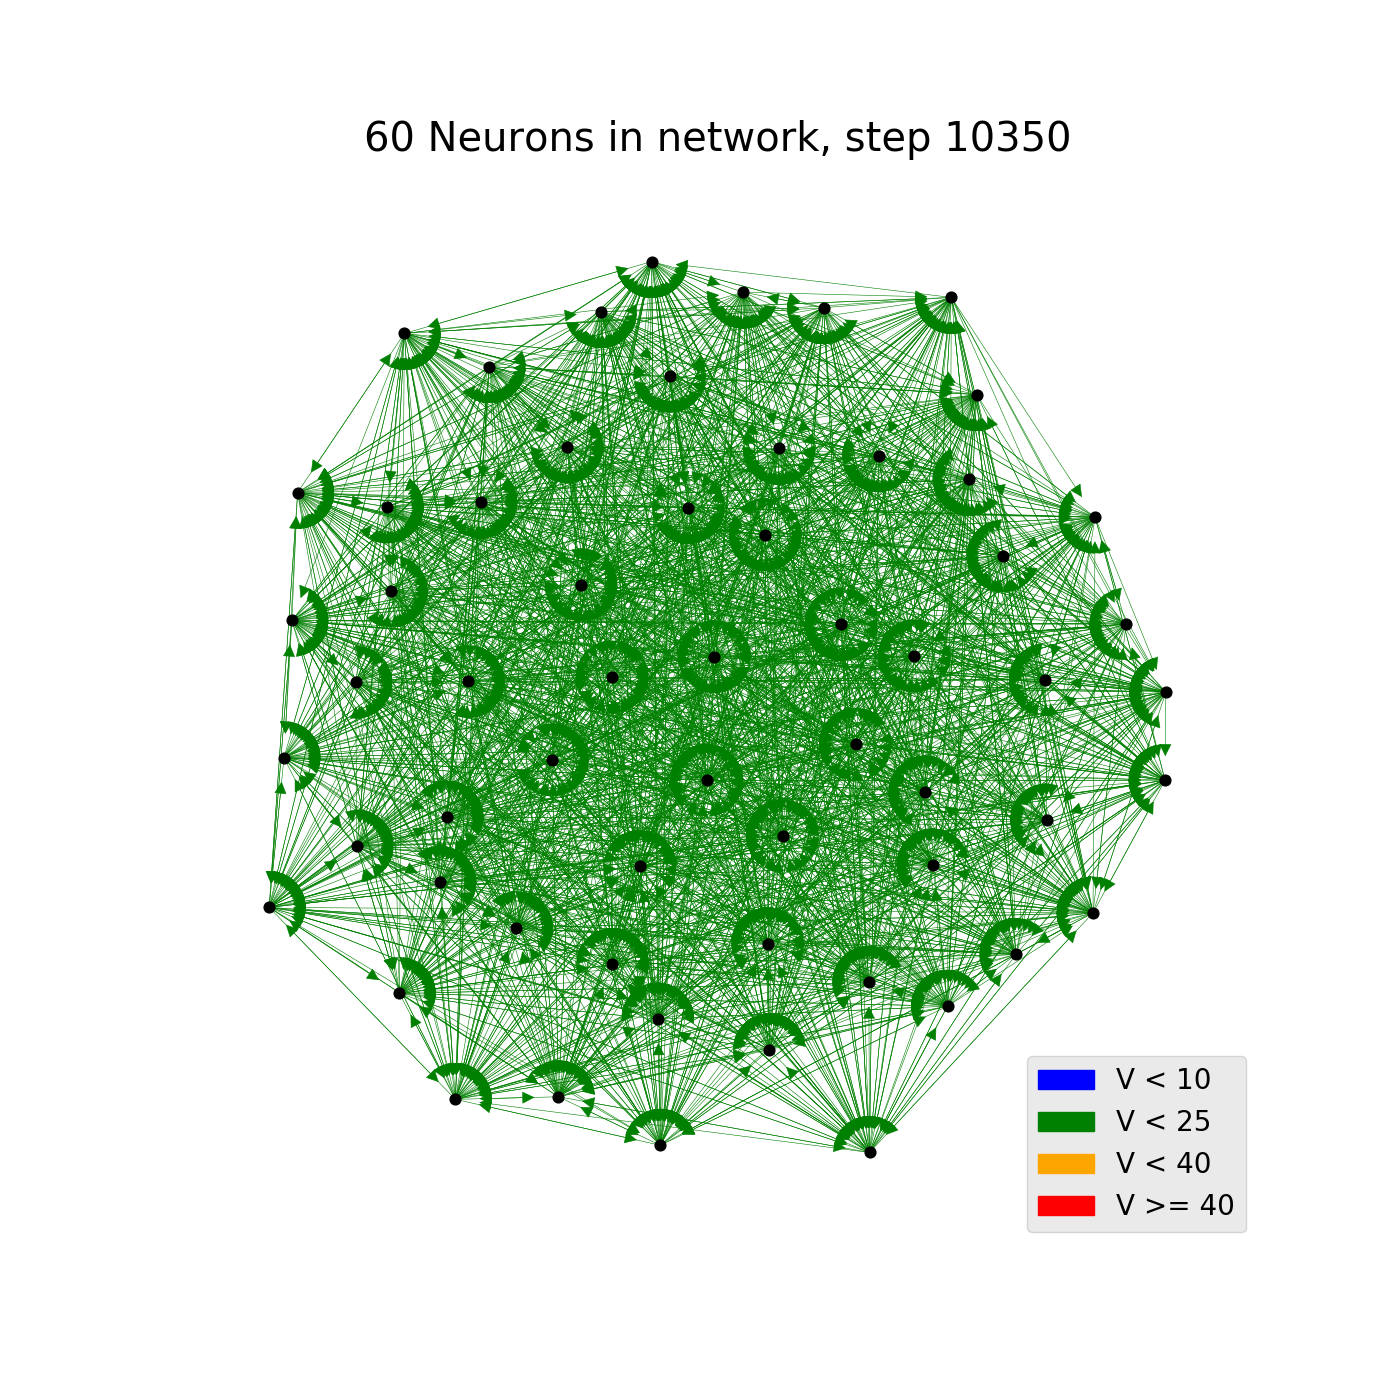
\includegraphics[width=40mm]{neuron_connectivity_at_step_10350}
  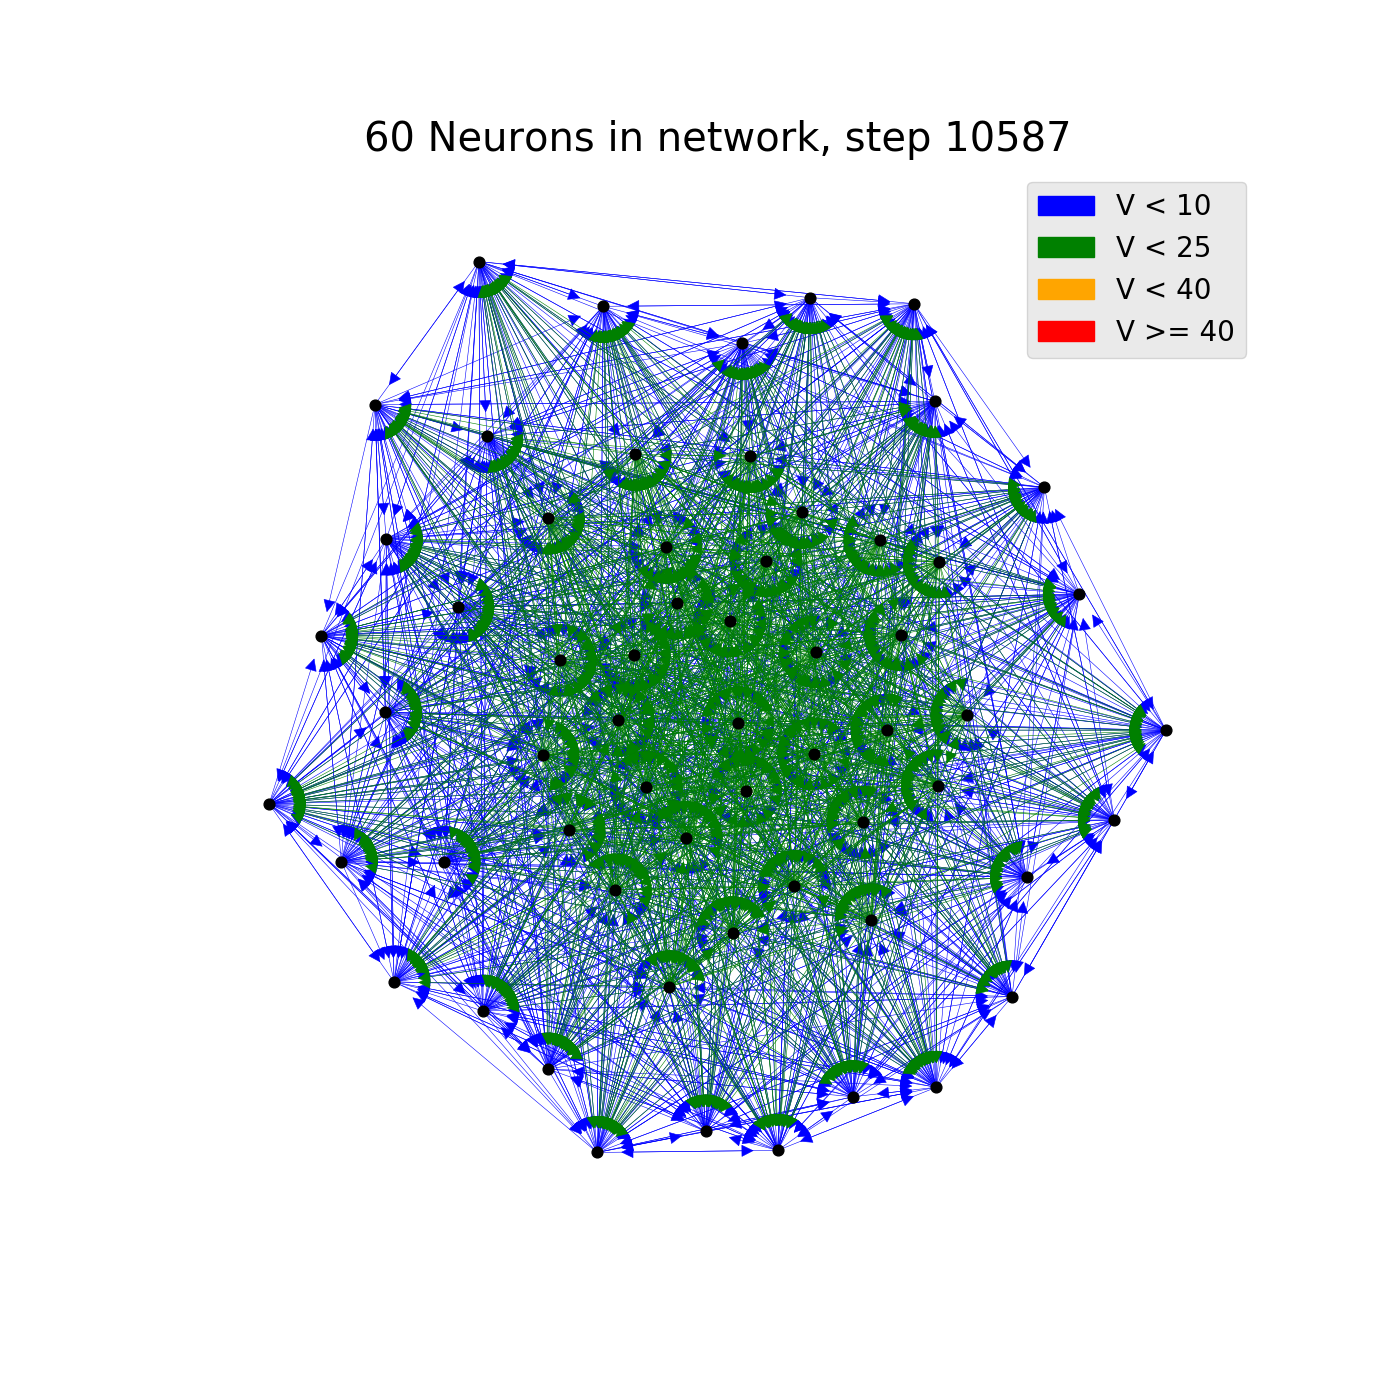
\includegraphics[width=40mm]{neuron_connectivity_at_step_10587}
  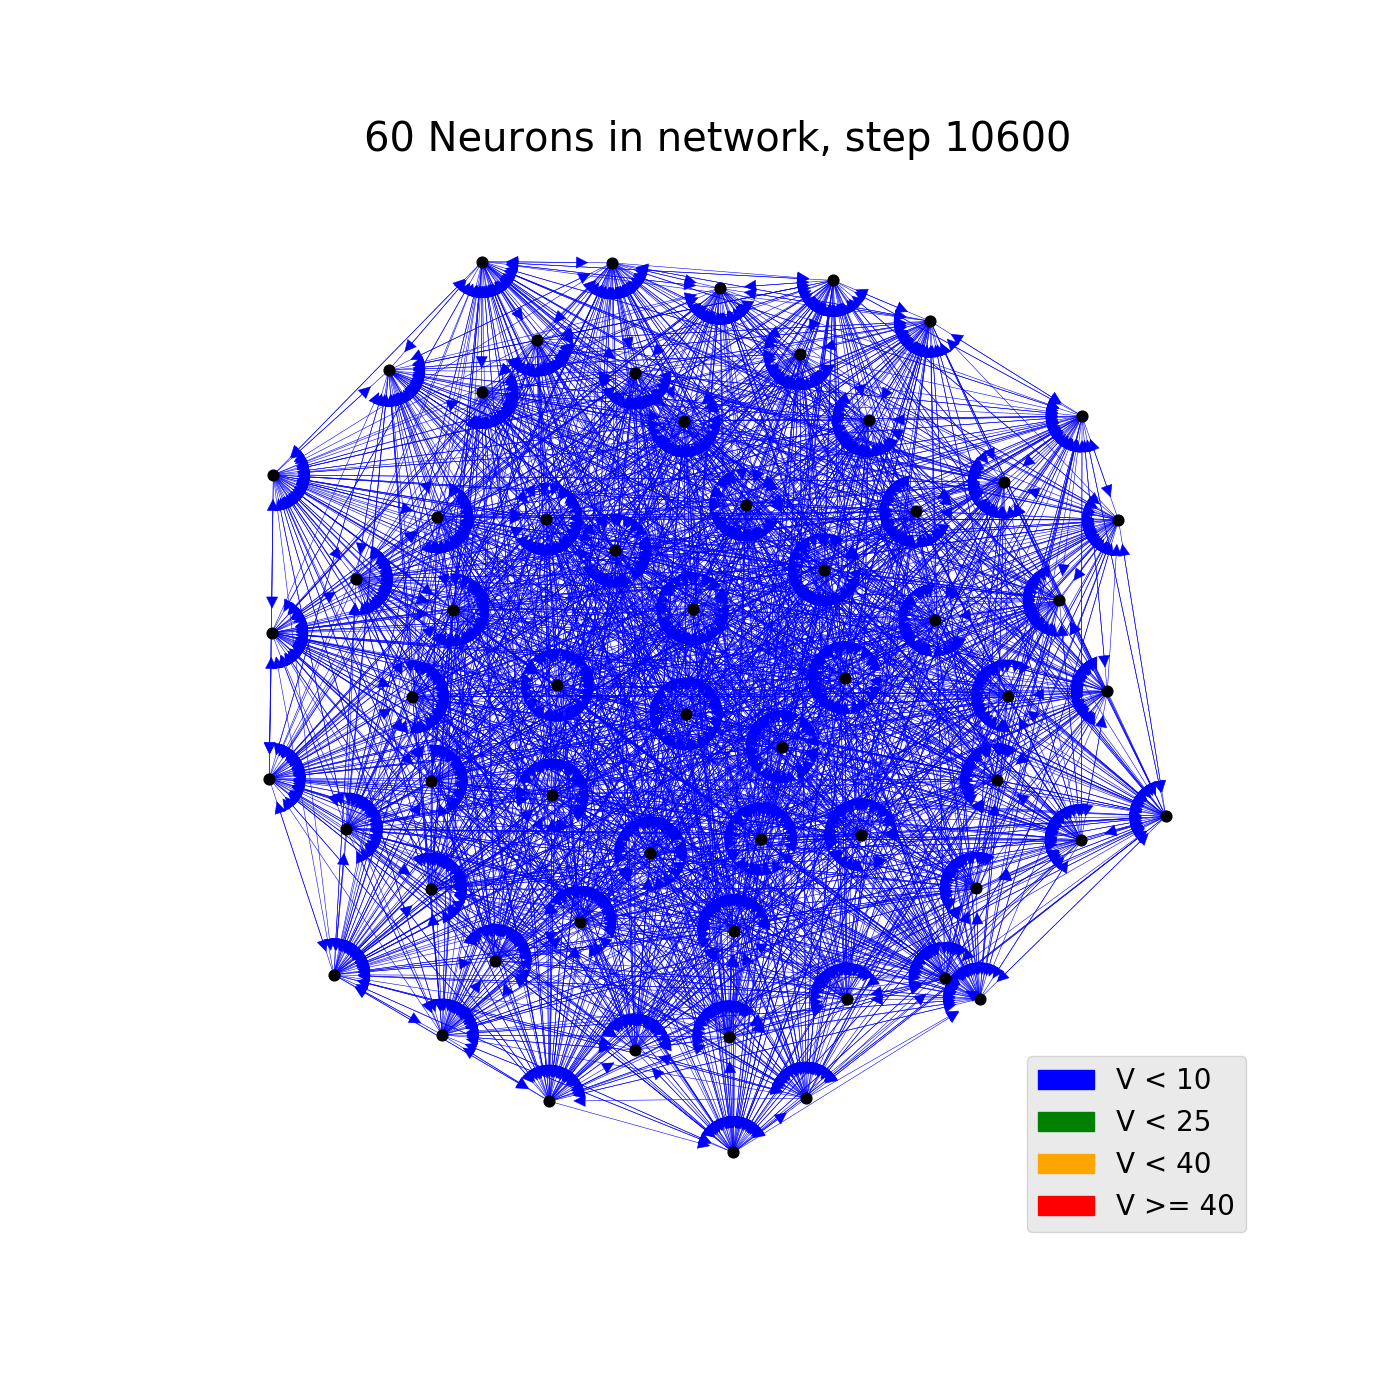
\includegraphics[width=40mm]{neuron_connectivity_at_step_10600}

  \caption{One cycle of heterogeneous network firing, beginning from basal firing rate, up to maximal firing rate, then relaxing again to basal firing rate.}
\end{figure}

\section{K-Core examples}
\label{appendix:kcore_examples}
\begin{figure}[!htb]
	\centering
    	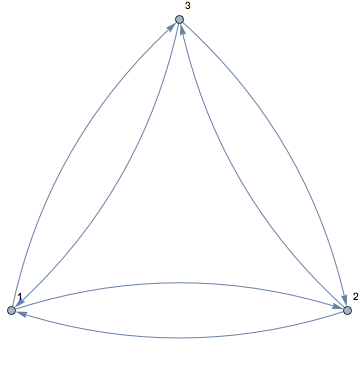
\includegraphics[width=40mm]{g1.png}
        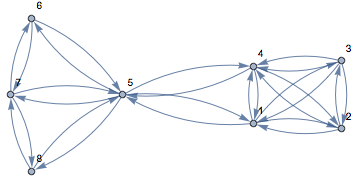
\includegraphics[width=70mm]{g2.png}
        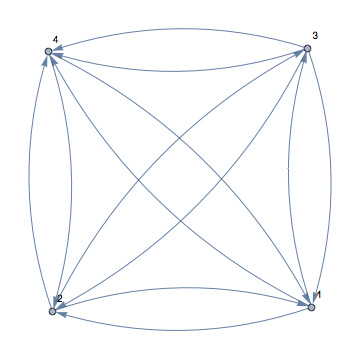
\includegraphics[width=45mm]{g3.png}
    \caption{Examples of k-cores. Left: Example of a 2-core of size 3. Center: Example of 3-core of size 4. Right: 3-Core of center network isolated from rest of network.}
\end{figure}

\end{appendices}

\end{document}
